% small.tex
\documentclass[10pt]{beamer}
\usetheme{amcg}
\beamertemplatenavigationsymbolsempty
\renewcommand{\thefootnote}{}
\providecommand{\e}[1]{\ensuremath{\times 10^{#1}}}
\usepackage{mathptmx}
\usepackage{helvet}
\newcommand\TILDE{\char`\~}
\usepackage{subfigure}
\usepackage{listings}

% items enclosed in square brackets are optional
\title[Introduction to the examples]{Introduction to the examples}
\subtitle[]{}
\institute{Department of Earth Science and Engineering, Imperial College London}
\author[Richard Ferrier]{\large{Richard Ferrier}}
\date{}
\AtBeginSection[]
{
  \begin{frame}
    \frametitle{Outline}
    \tableofcontents[currentsection]
  \end{frame}
}

\begin{document}

%--- the titlepage frame -------------------------%
\begin{frame}
  \titlepage
\end{frame}

%-- Overview slide --- %
\section*{Outline}
\begin{frame}
  \frametitle{Outline}
  \tableofcontents
\end{frame}

\section{CFD Examples}

%\documentclass[10pt]{beamer}
%\usetheme{amcg}
%\usepackage{subfigure}

%\begin{document}

\subsection{Advection of a top hat}

\begin{frame}
  \frametitle{Advection of a top hat}
  \begin{itemize}
  \item Top hat distribution of a tracer, advected with prescribed velocity
  \item Compares CG, CV, DG discretisations
  \item Simple, fast: run time 2 min.
  \end{itemize}

  \begin{figure}
    \centering
    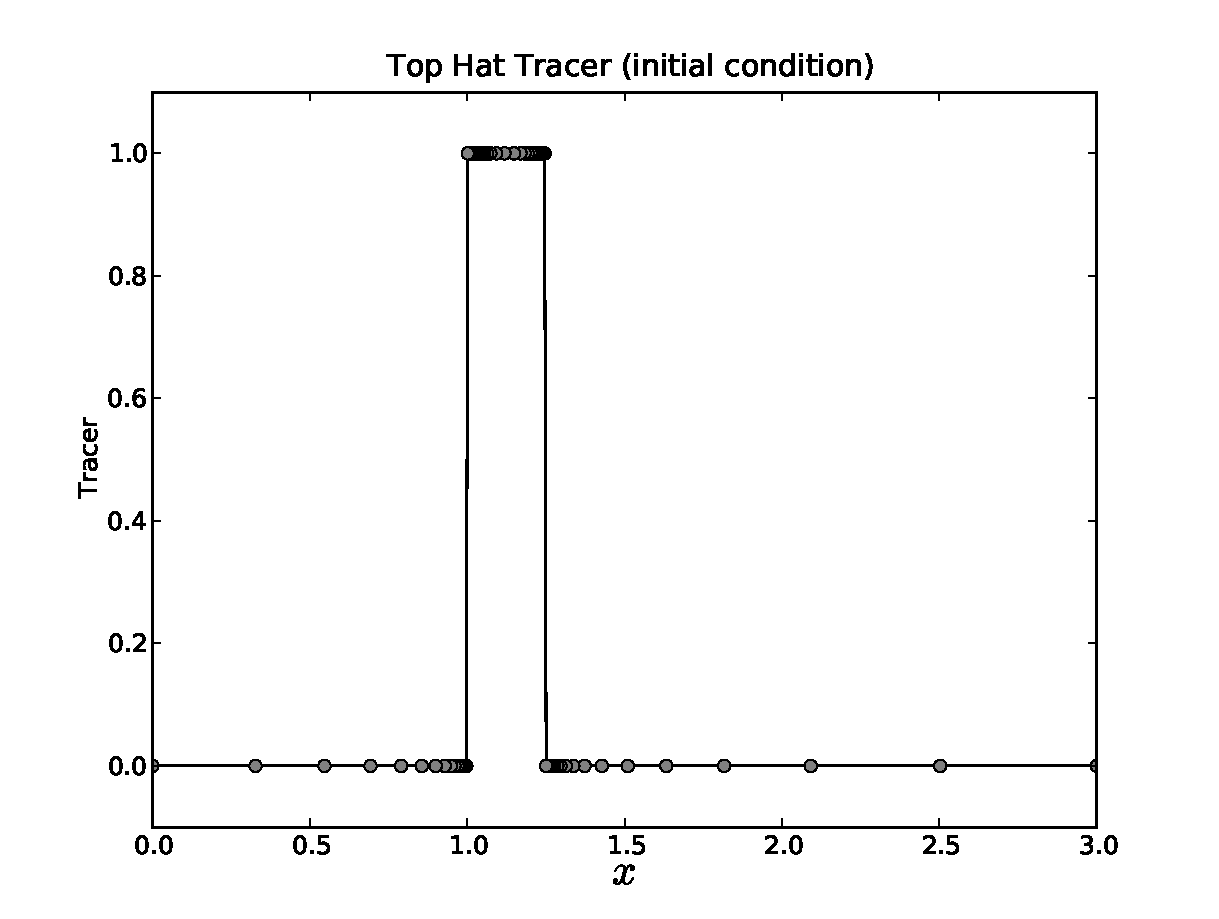
\includegraphics[width=0.45\textwidth]{./top_hat/top_hat_ic.pdf}
    \caption{Initial top hat distribution.}
  \end{figure}
\end{frame}

\begin{frame}
  \frametitle{Advection of a top hat}
  \begin{figure}[ht]
    \begin{tabular}{ccc}
      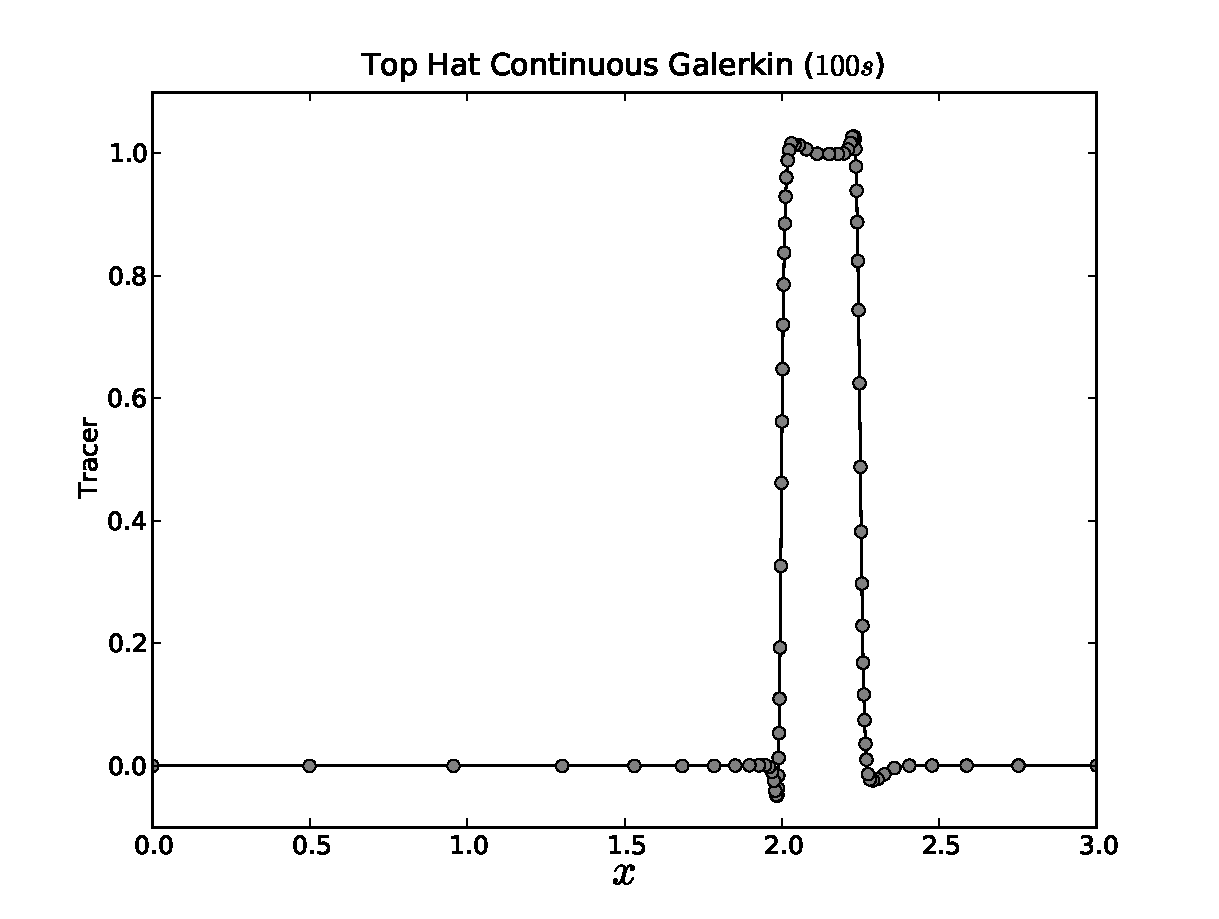
\includegraphics[width=0.3\textwidth]{./top_hat/top_hat_cg.pdf} &
      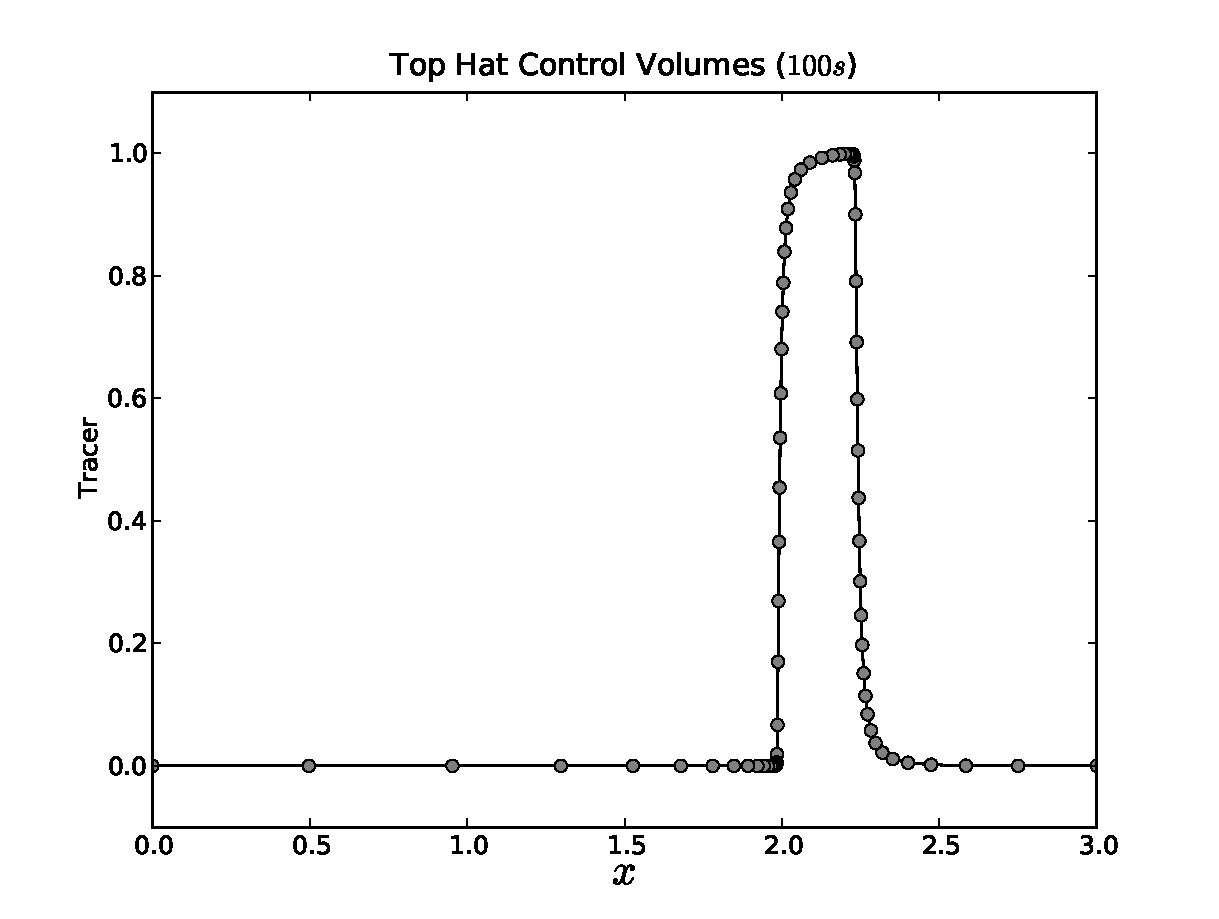
\includegraphics[width=0.3\textwidth]{./top_hat/top_hat_cv.pdf} &
      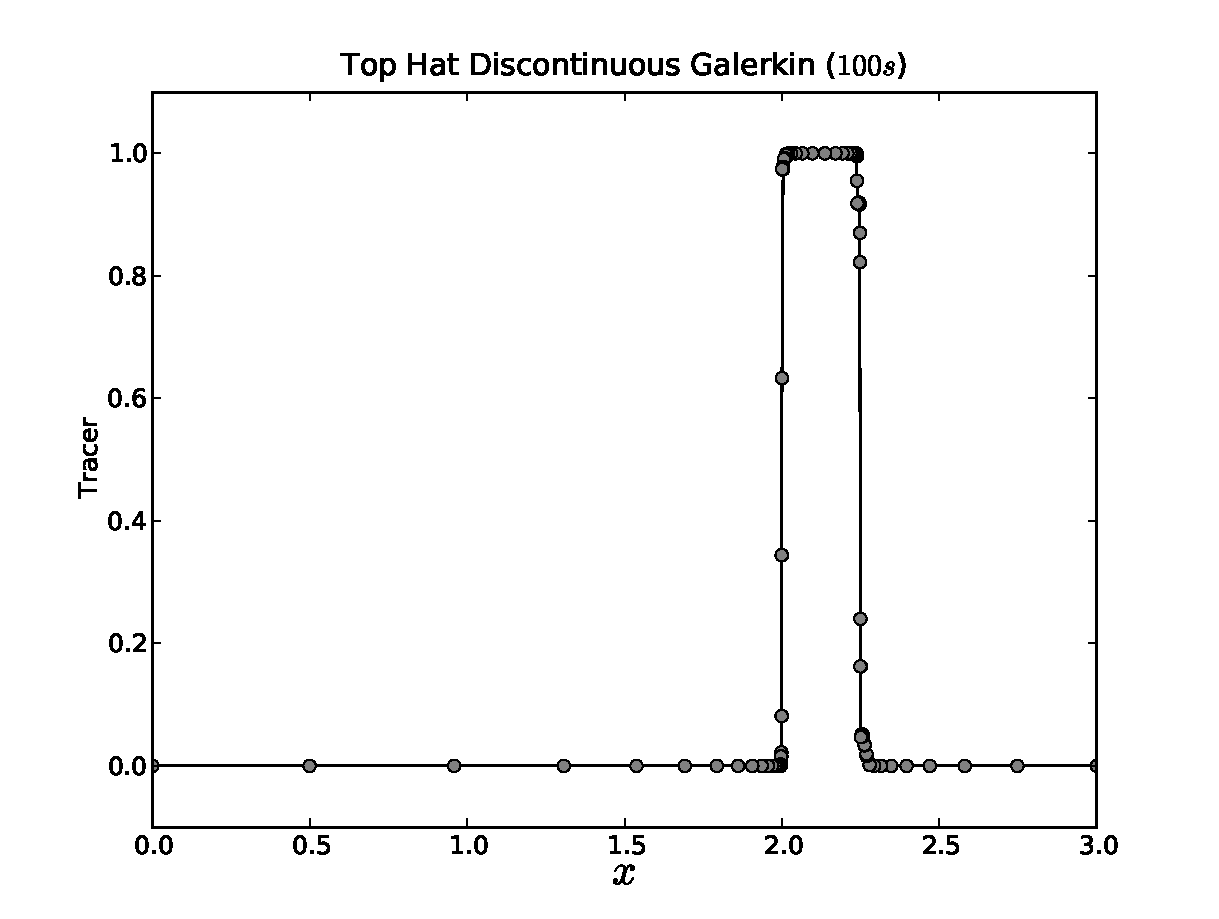
\includegraphics[width=0.3\textwidth]{./top_hat/top_hat_dg.pdf} \\
      Continuous & Control & Discontinuous  \\
       Galerkin &  Volume & Galerkin
    \end{tabular}
  \end{figure}
\end{frame}

\begin{frame}
  Continuous Galerkin
  \begin{itemize}
  \item Basic finite element discretisation
  \item Not good for advection of sharp discontinuities
  \item Not conservative
  \item SUPG stabilisation applied in this instance
  \end{itemize}
  \vspace{5pt}
  Control Volume
  \begin{itemize}
  \item Simple and efficient, sometimes diffusive
  \item Need to choose an interpolation method.  Here, `FiniteElement' interpolation with Sweby limiter is used.
  \end{itemize}
  \vspace{5pt}
  Discontinuous Galerkin
  \begin{itemize}
  \item Popular for advection problems
  \item Slope limiters still needed near discontinuities to prevent overshoots
  \end{itemize}
\end{frame}

\begin{frame}
  \frametitle{Exercises}
  \begin{itemize}
    \item Turn off SUPG stabilisation for the CG case and see what it does.
    \item Change the resolution of the adapted meshes.
    \item Change the temporal and spatial discretisations to get a less diffusive CV advection scheme.
  \end{itemize}
\end{frame}

%\end{document}

%-- Add sections and your outline will be created automatically --%
\section{Lid--Driven Cavity}

% Frame starts a new slide
\begin{frame}
    \frametitle{Lid--Driven Cavity}
\begin{itemize}
\item Simple test case often used for verification and validation
\item Re = 1000
\end{itemize}
\begin{figure}
\centering
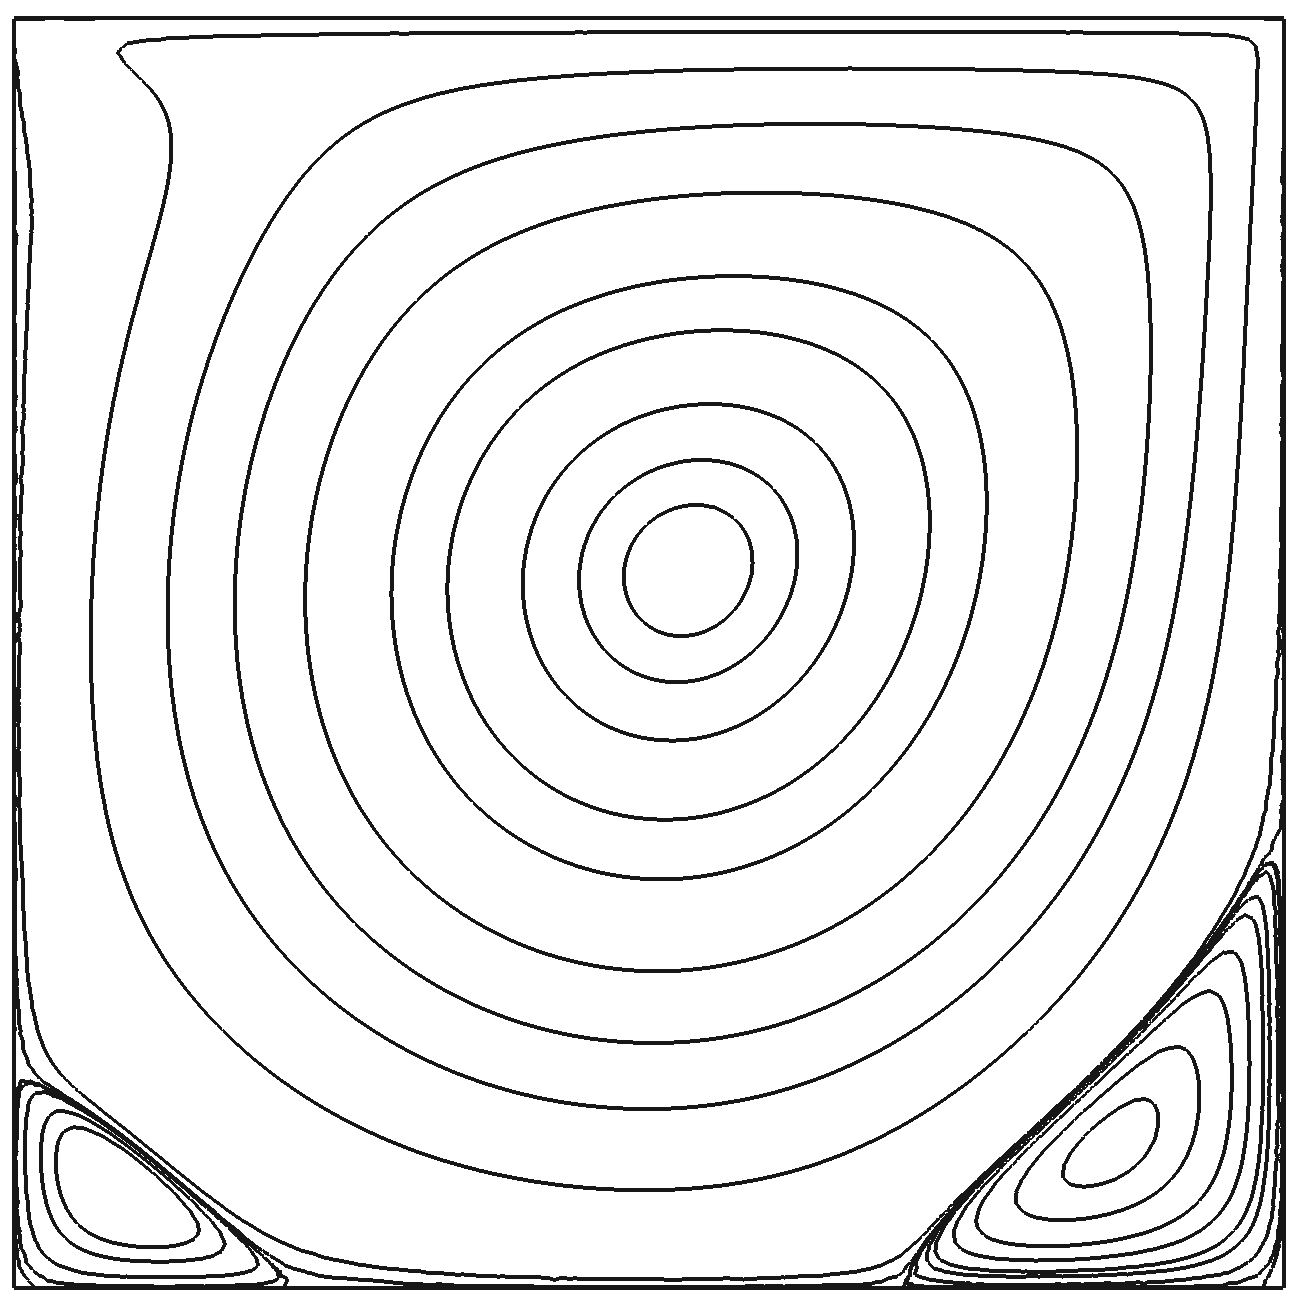
\includegraphics[width=0.4\textwidth]{./driven_cavity/driven_cavity_streamfunction.png}
\caption{Streamfunction contours in converged solution for $h=1/128$.}
\end{figure}
% end my slide
\end{frame}

\begin{frame}
    \frametitle{Lid--Driven Cavity}
\begin{figure}
\centering
\subfigure[vorticity contours in converged solution for \mbox{$h=1/128$}]{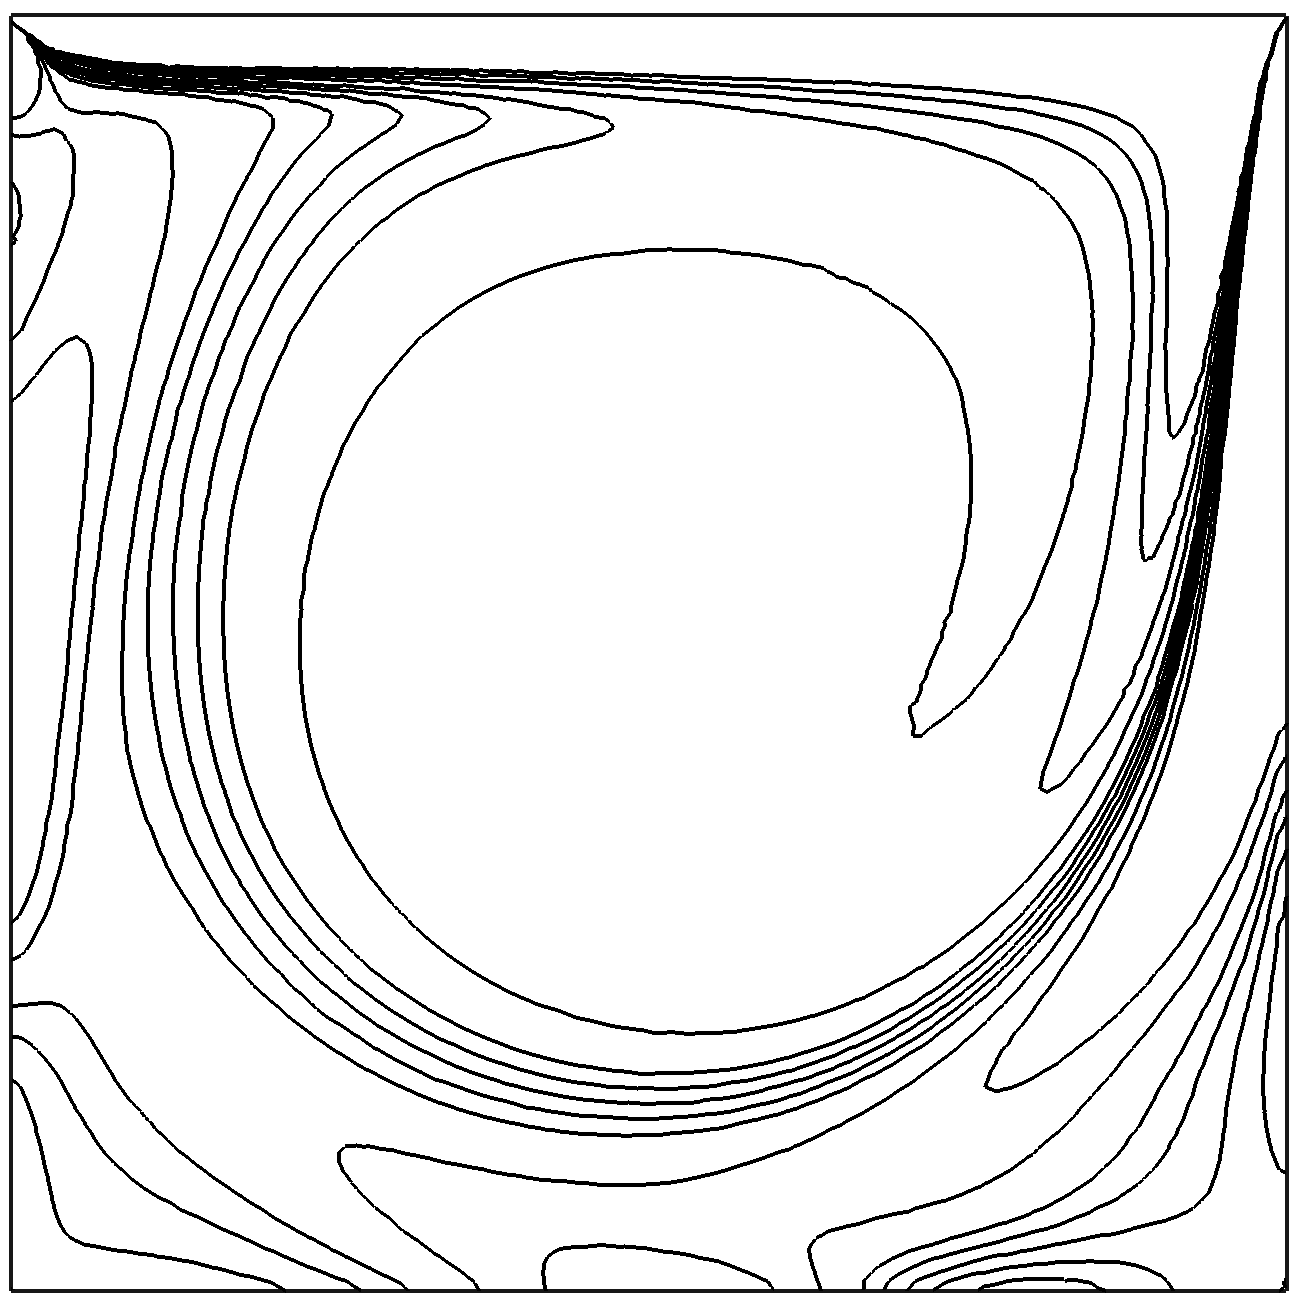
\includegraphics[width=0.35\textwidth]{./driven_cavity/driven_cavity_vorticity.png}}
\hspace{10mm}
\subfigure[error vs. experiment]{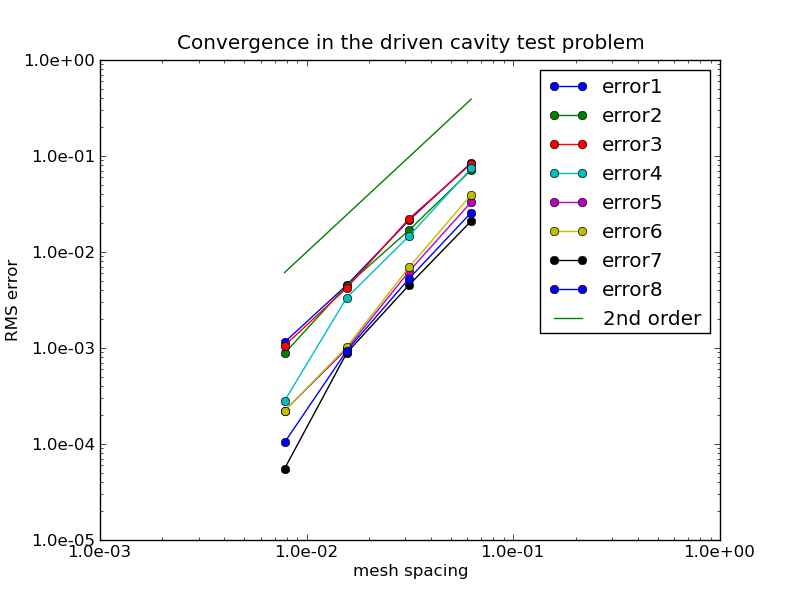
\includegraphics[width=0.45\textwidth]{./driven_cavity/driven_cavity_error_plot.png}}
\caption{The error metrics are listed in the manual.}
\end{figure}
\end{frame}





%-- Add sections and your outline will be created automatically --%
\subsection{Backward facing step}

\begin{frame}
    \frametitle{Backward facing step (2D and 3D)}
\begin{itemize}
\item Classic CFD test case
\item Experimental and numerical data available for comparison
\item Test of numerical methods or turbulence models
\end{itemize}
\begin{figure}
\centering
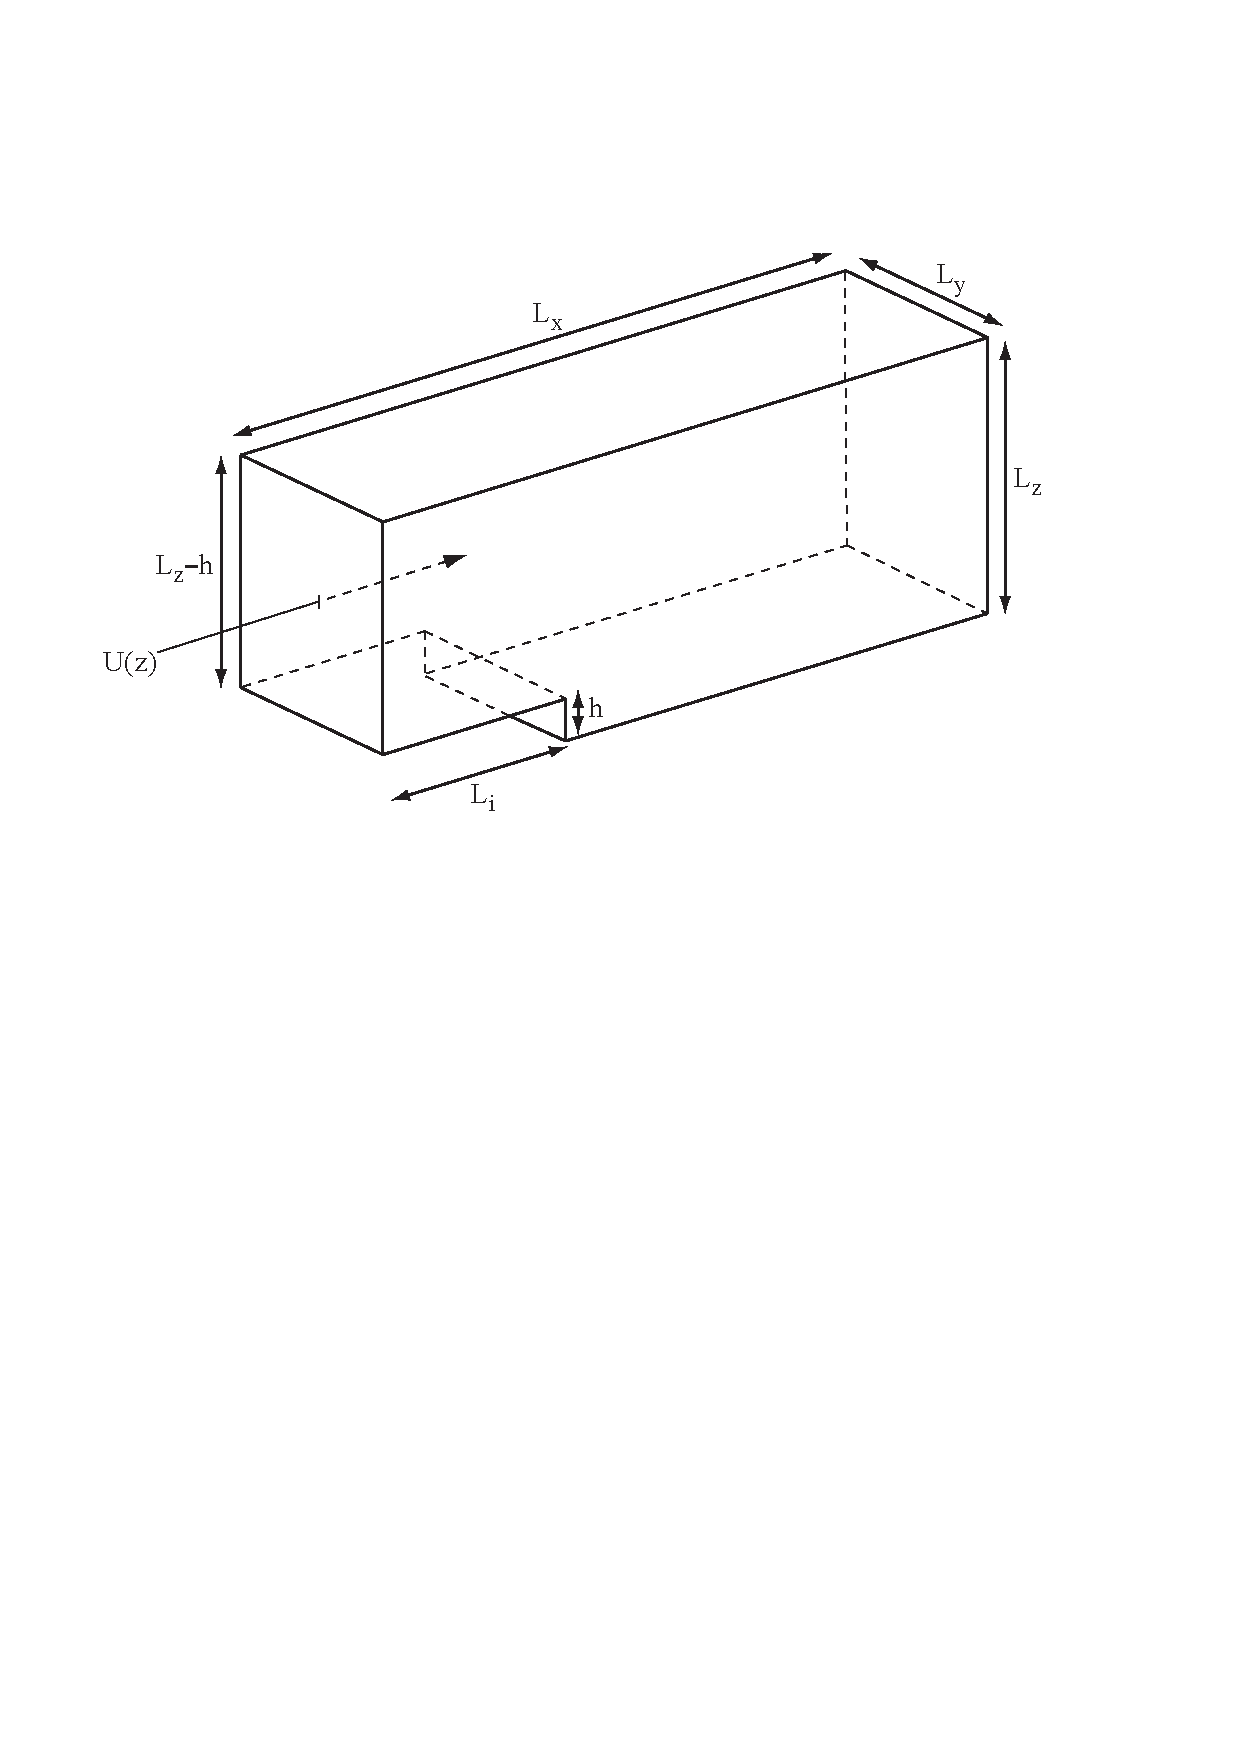
\includegraphics[width=0.5\textwidth]{./backward_facing_step/backward_facing_step_3d-schematic}
\caption{Geometry of 3D backward facing step}
\end{figure}
\end{frame}
%
\begin{frame}
    \frametitle{Backward facing step (2D and 3D)}
Run times: 
\begin{itemize}
\item 25 min. for 2D reference
\item 6 hr. for 2D with k-$\epsilon$
\item 5 hr. (8 cpu) for 3D
\end{itemize}
\begin{figure}
\centering
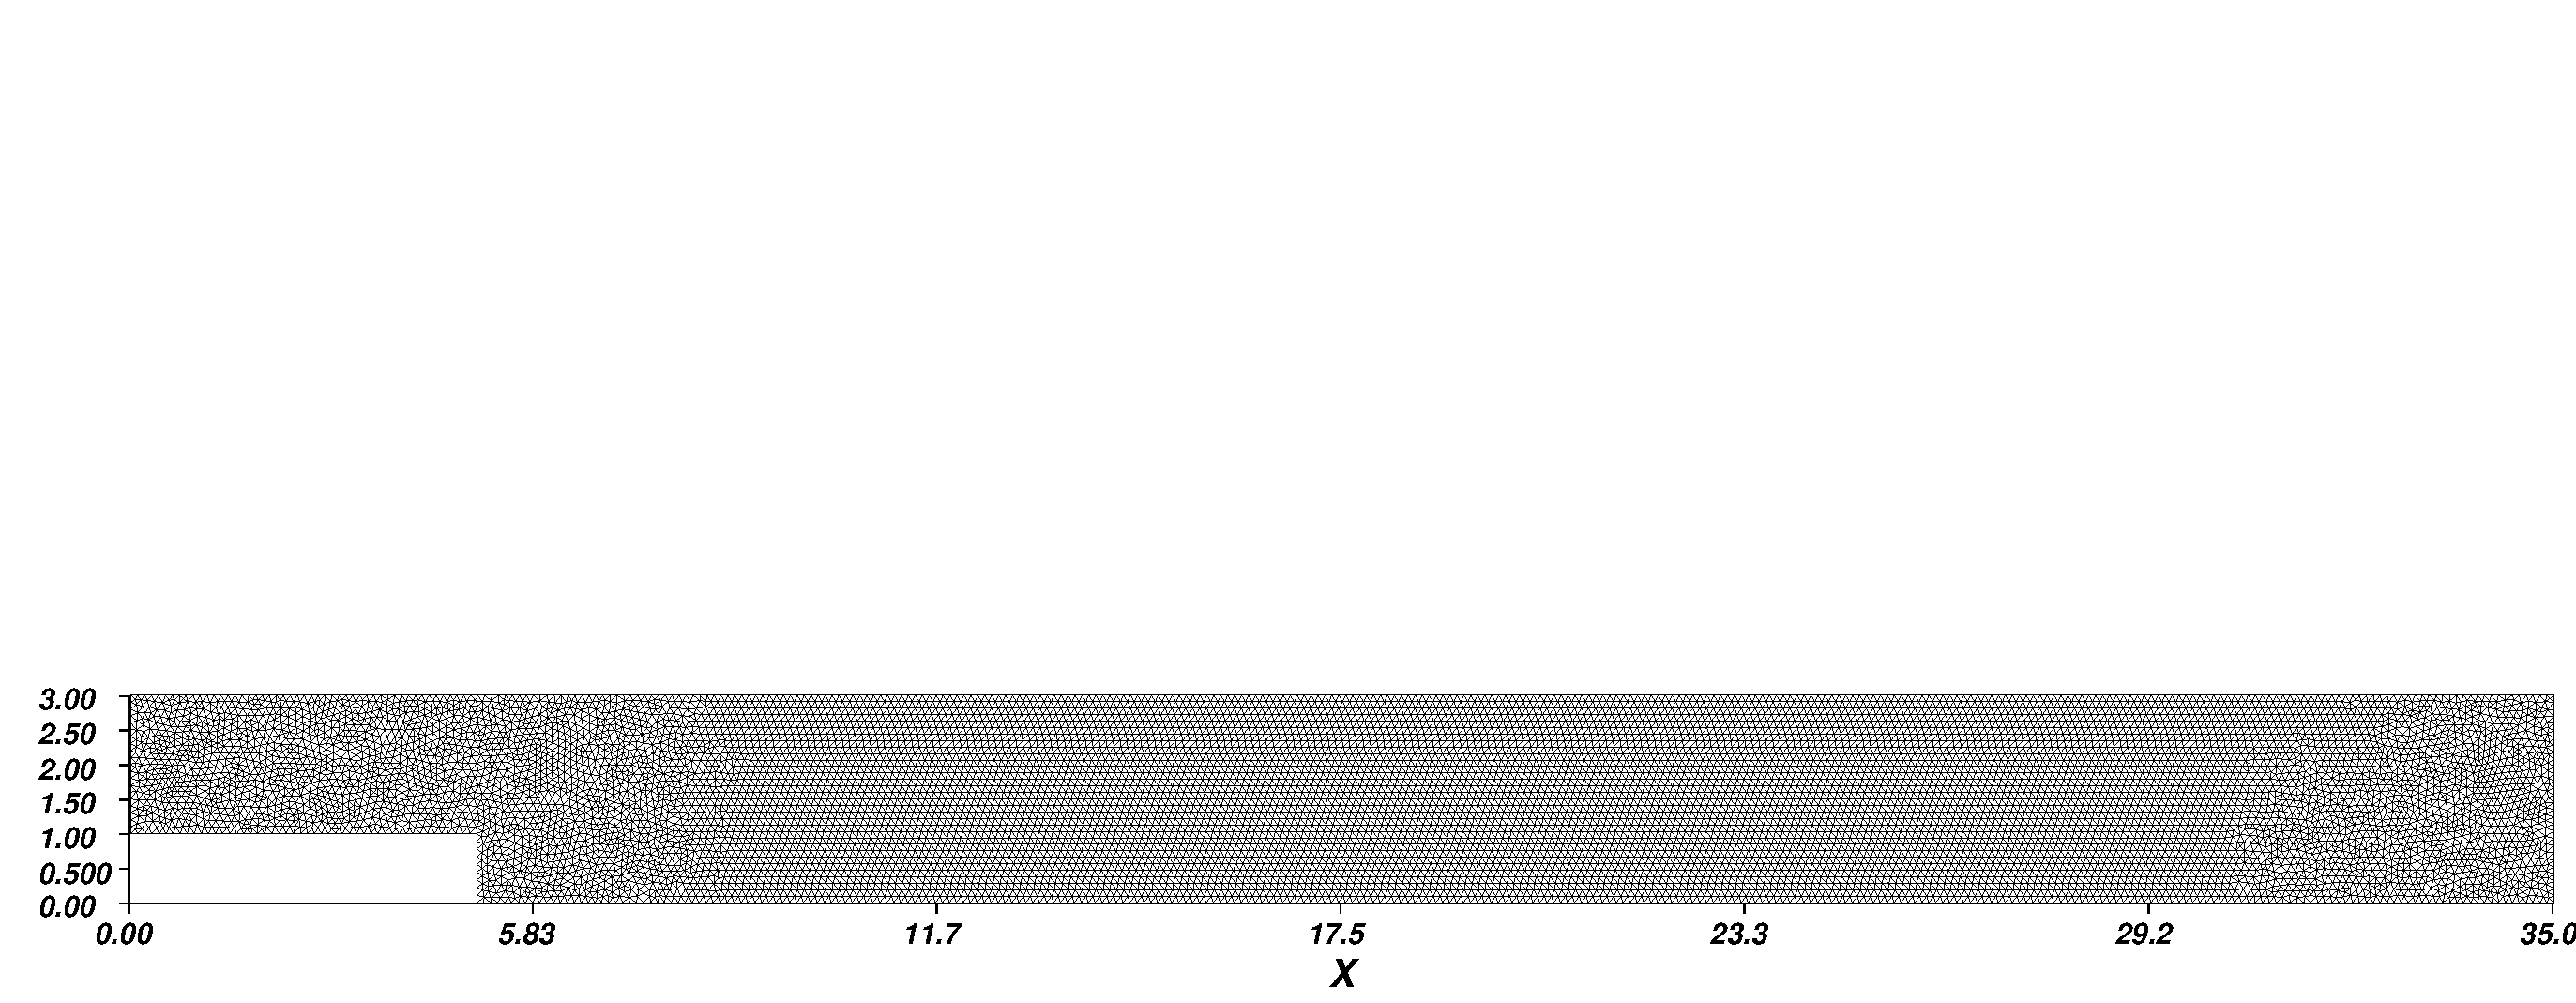
\includegraphics[width=1.0\textwidth]{./backward_facing_step/backward_facing_step_2d-mesh}
\caption{Geometry of 2D backward facing step showing the mesh.}
\end{figure}
\end{frame}
%
\begin{frame}
    \frametitle{Backward facing step, 2D results}
\begin{itemize}
\item Reattachment point estimation
\item Profile evolution in time/space
\end{itemize}
\begin{figure}
\centering
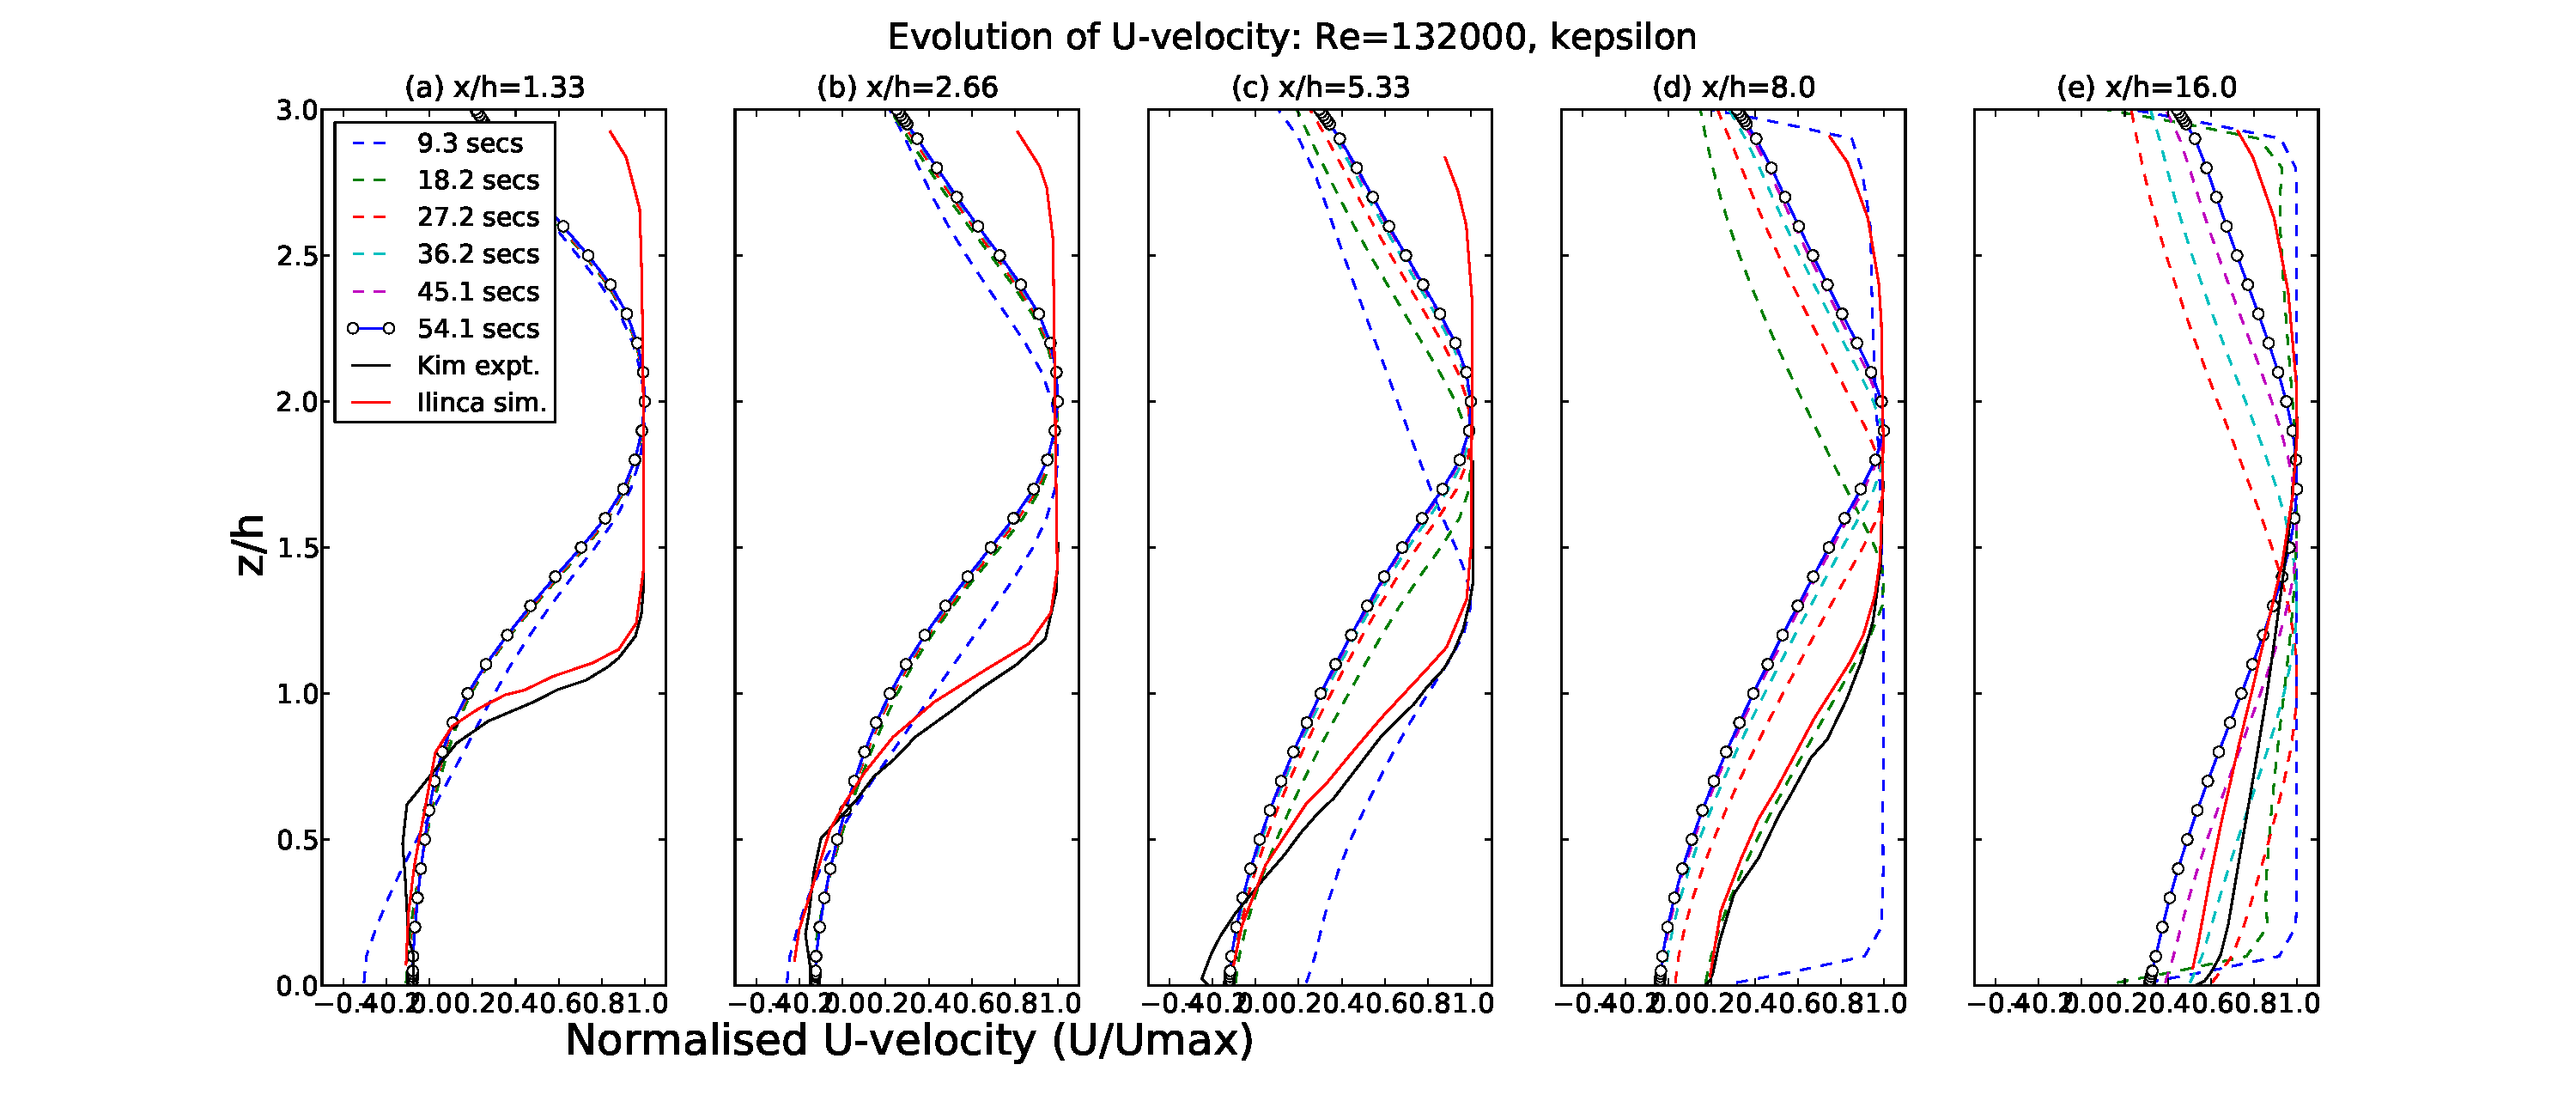
\includegraphics[width=0.7\textwidth]{./backward_facing_step/velocity_profiles_kim_kepsilon}
\caption{Streamwise velocity profiles at several points downstream of the step showing the converged solution and comparing to experimental and other numerical data.}
\end{figure}

\end{frame}
%
\begin{frame}
    \frametitle{Backward facing step, 3D results}
\begin{itemize}
\item Recirculation bubble and reattachment point
\end{itemize}

\begin{figure}
\centering
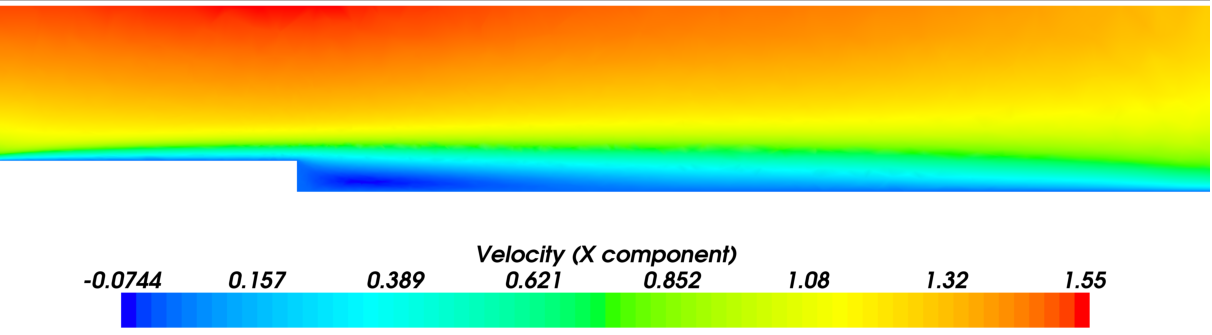
\includegraphics[width=0.8\textwidth]{./backward_facing_step/velo-magnitude-3d-50sec}
\caption{Velocity cut plane through centre of 3D geometry, time $=50\,$s.}
\end{figure}

\end{frame}
%
\begin{frame}
    \frametitle{Backward facing step, exercises}
\begin{itemize}
\item Increase the Reynolds number.
\item Add adaptivity options.
\end{itemize}

\end{frame}

%-- Add sections and your outline will be created automatically --%
\subsection{Flow past a sphere}

% Frame starts a new slide
\begin{frame}
    \frametitle{Flow past a sphere}
\begin{itemize}
\item Drag calculation at different Reynolds numbers
\item Adaptive mesh resolves dynamics near surface
%\item Option: \option{Velocity/stat/compute\_body\_forces\_on\_surfaces}
\end{itemize}
\begin{figure}
\centering
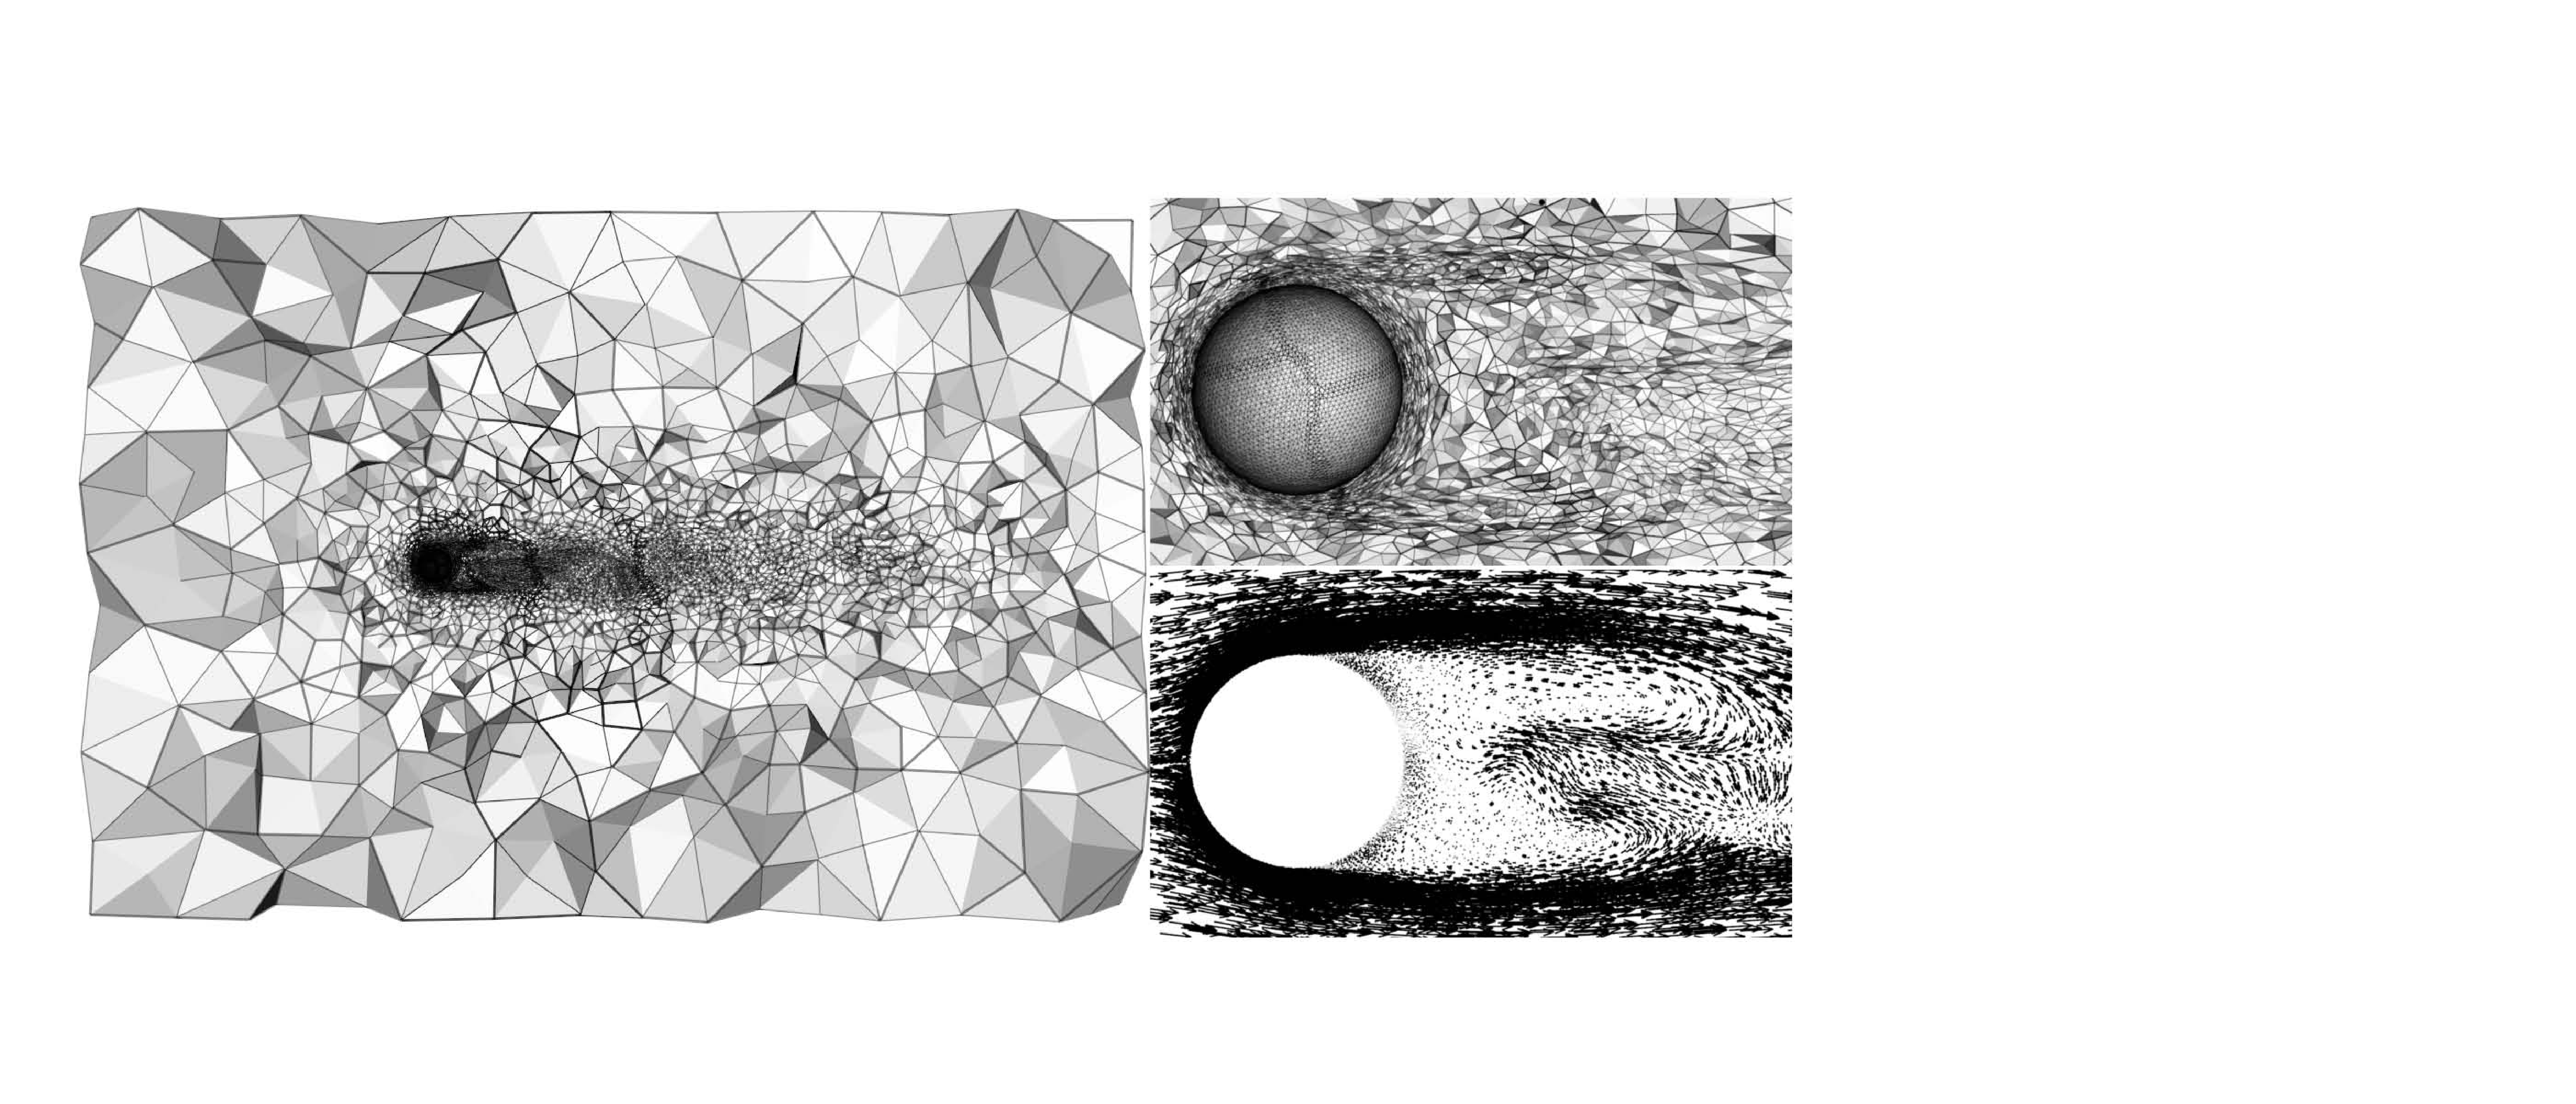
\includegraphics[width=0.8\textwidth]{./flow_past_sphere/sphere-Re1000-combined.pdf}
\caption{Sphere at $Re = 1000$. Clockwise from left: Cut plane showing anisotropic mesh, close up of sphere, velocity vectors.}
\end{figure}
\end{frame}

\begin{frame}
    \frametitle{Flow past a sphere}
\begin{itemize}
\item Plot streamlines by processing vtu files in Paraview
\item Time series of pressure and viscous drag force integrals available in stat file
%\item Option: \option{Velocity/stat/compute\_body\_forces\_on\_surfaces}
\end{itemize}
\begin{figure}
\centering
\subfigure[Re = 1]{
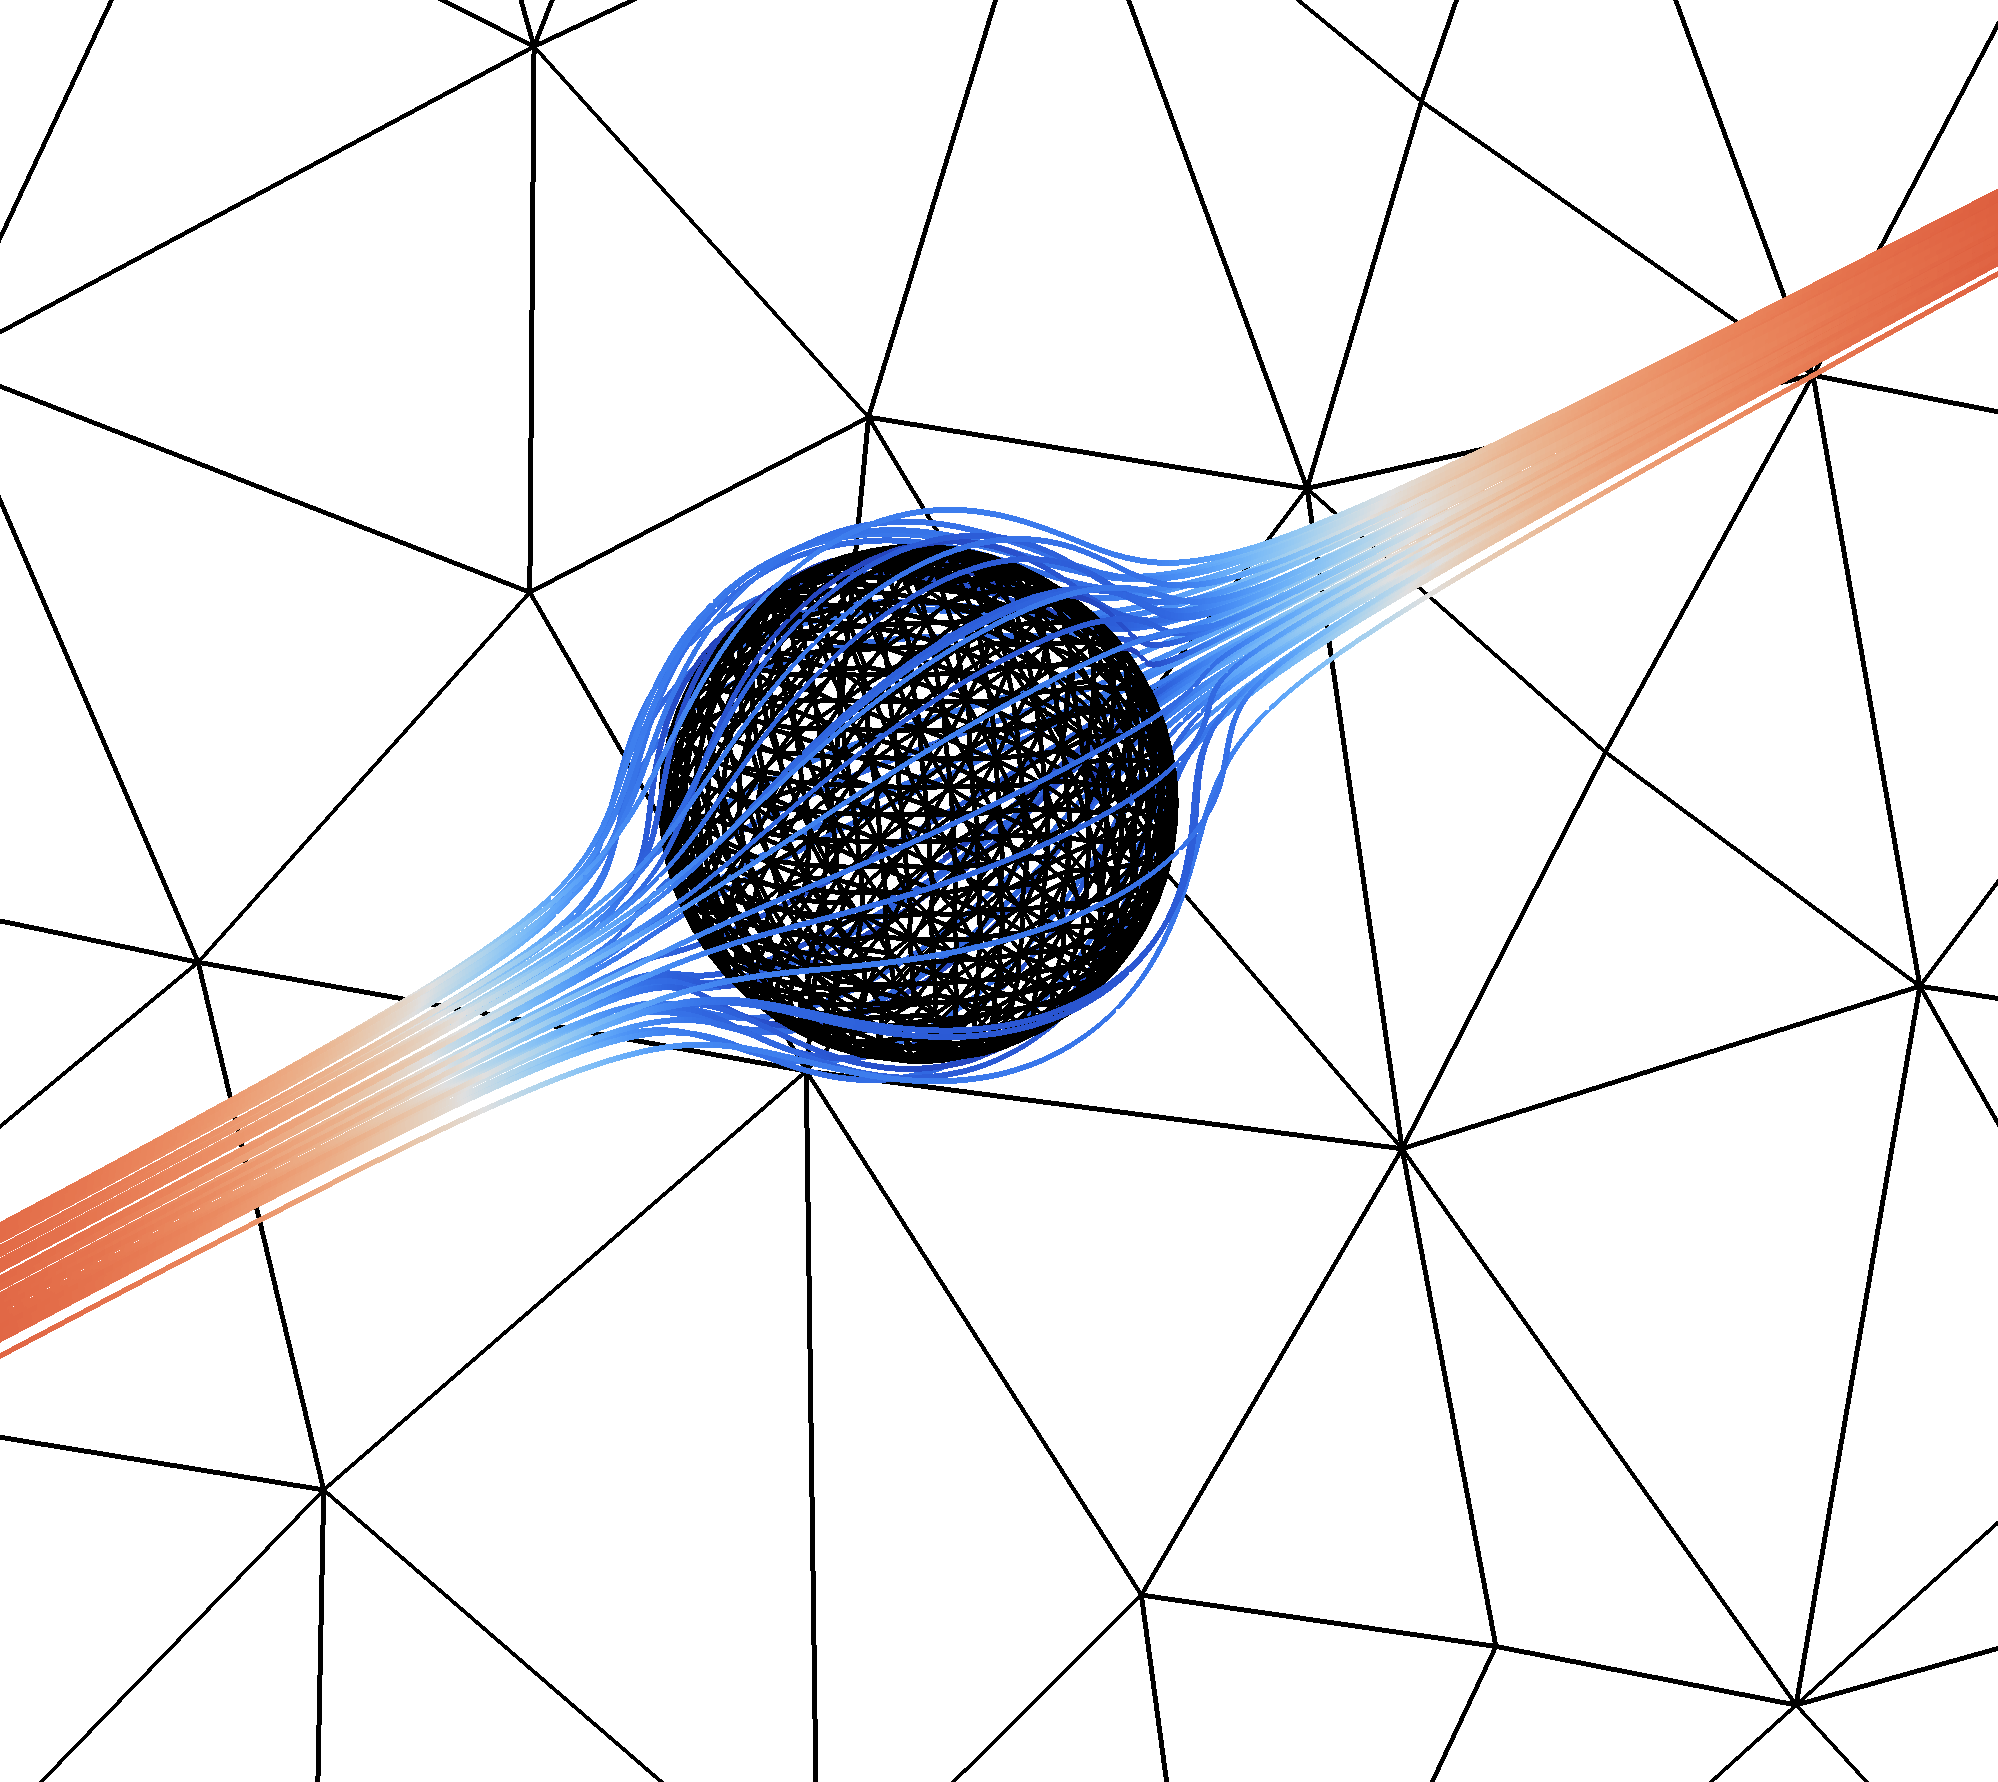
\includegraphics[width=0.225\textwidth]{./flow_past_sphere/sphere-Re1-streamlines.png}}
\subfigure[Re = 10]{
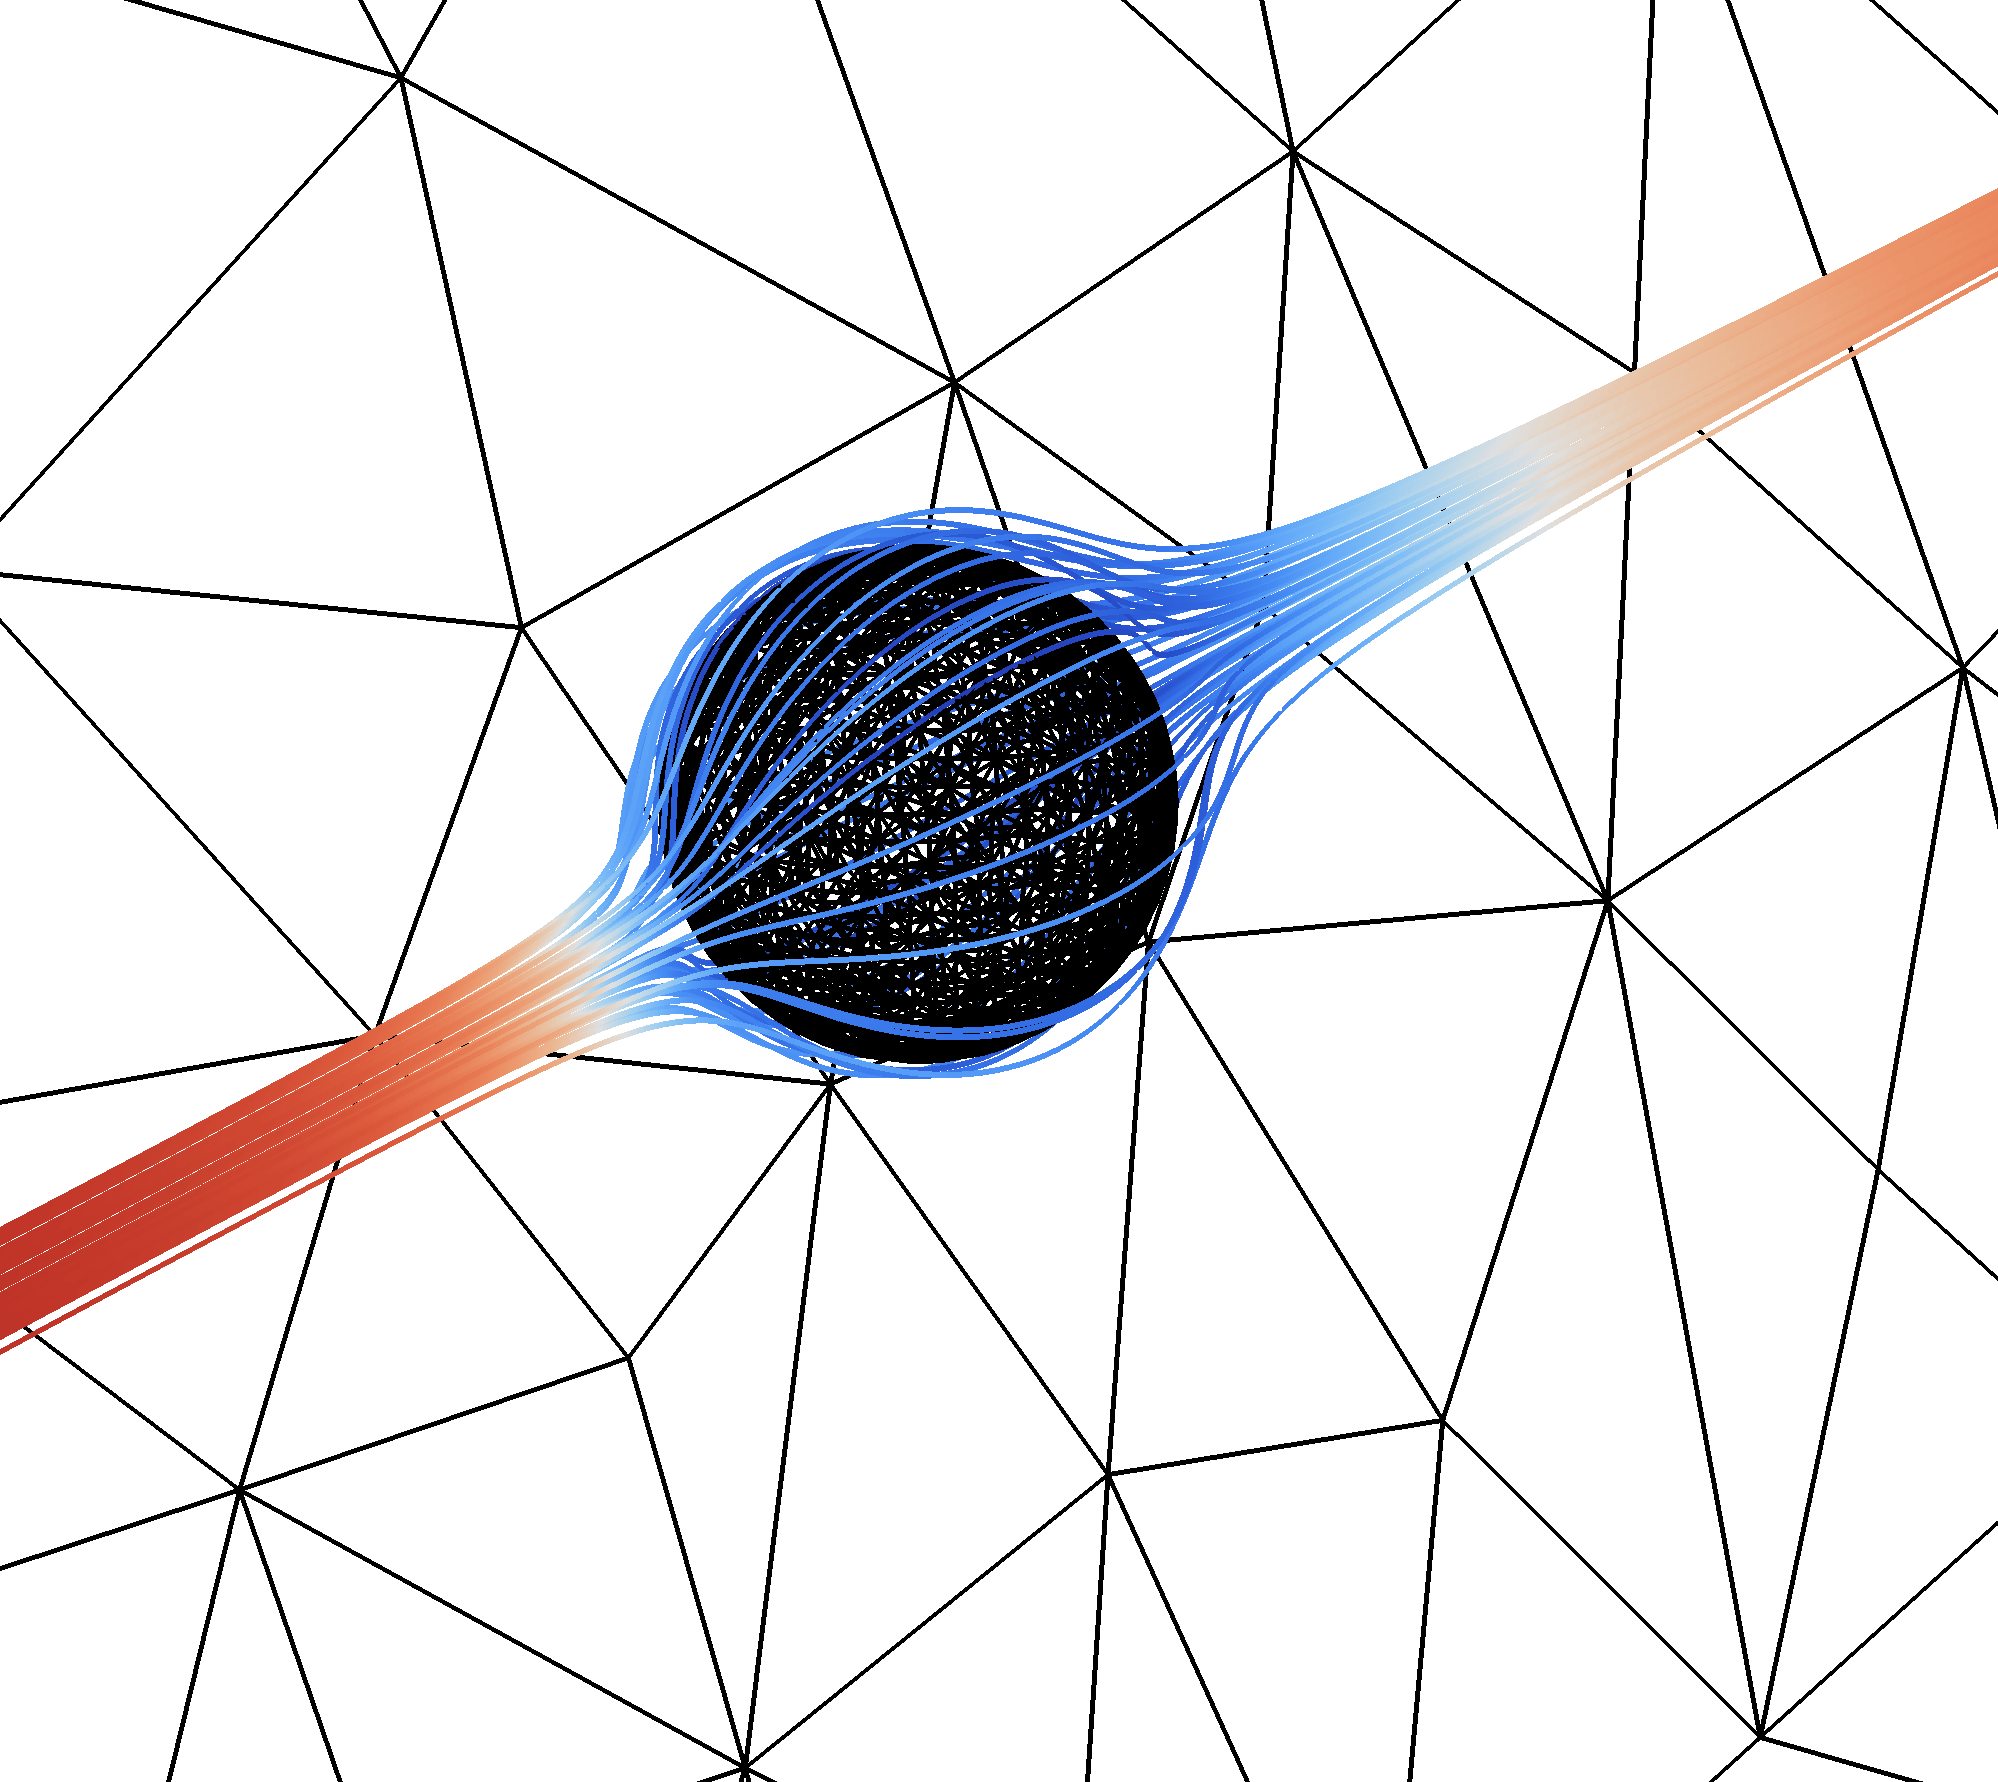
\includegraphics[width=0.225\textwidth]{./flow_past_sphere/sphere-Re10-streamlines.png}}
\subfigure[Re = 100]{
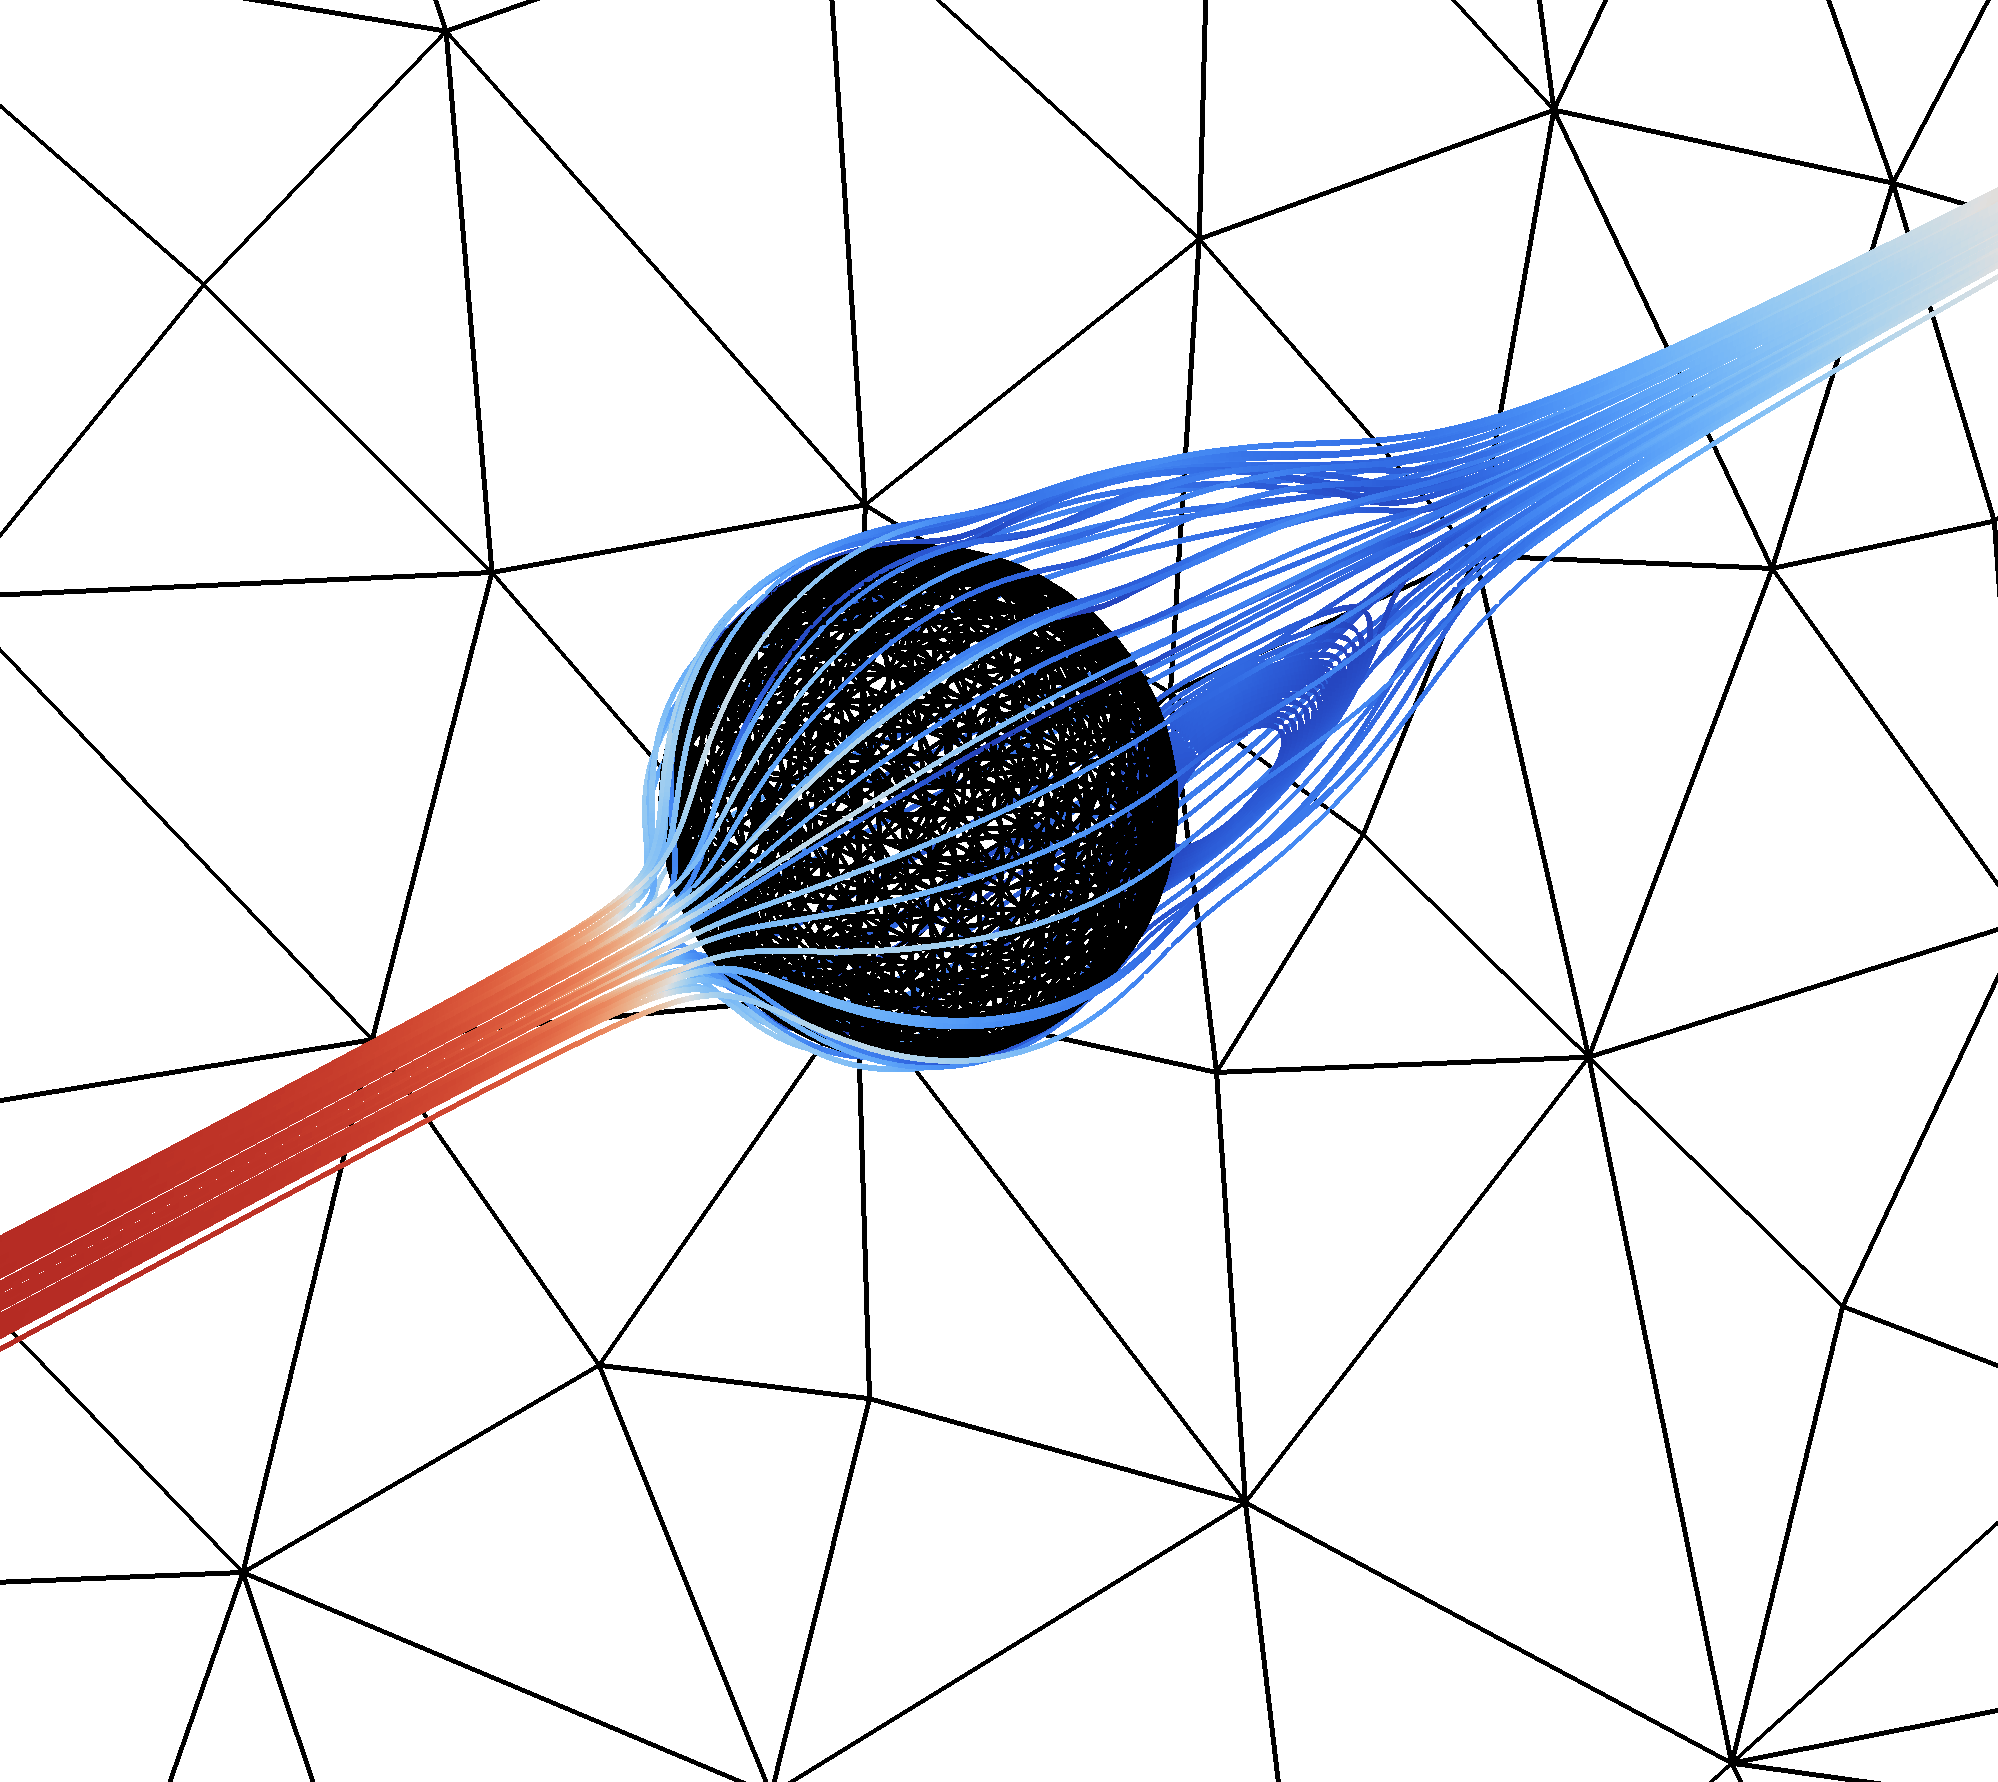
\includegraphics[width=0.225\textwidth]{./flow_past_sphere/sphere-Re100-streamlines.png}}
\subfigure[Re = 1000]{
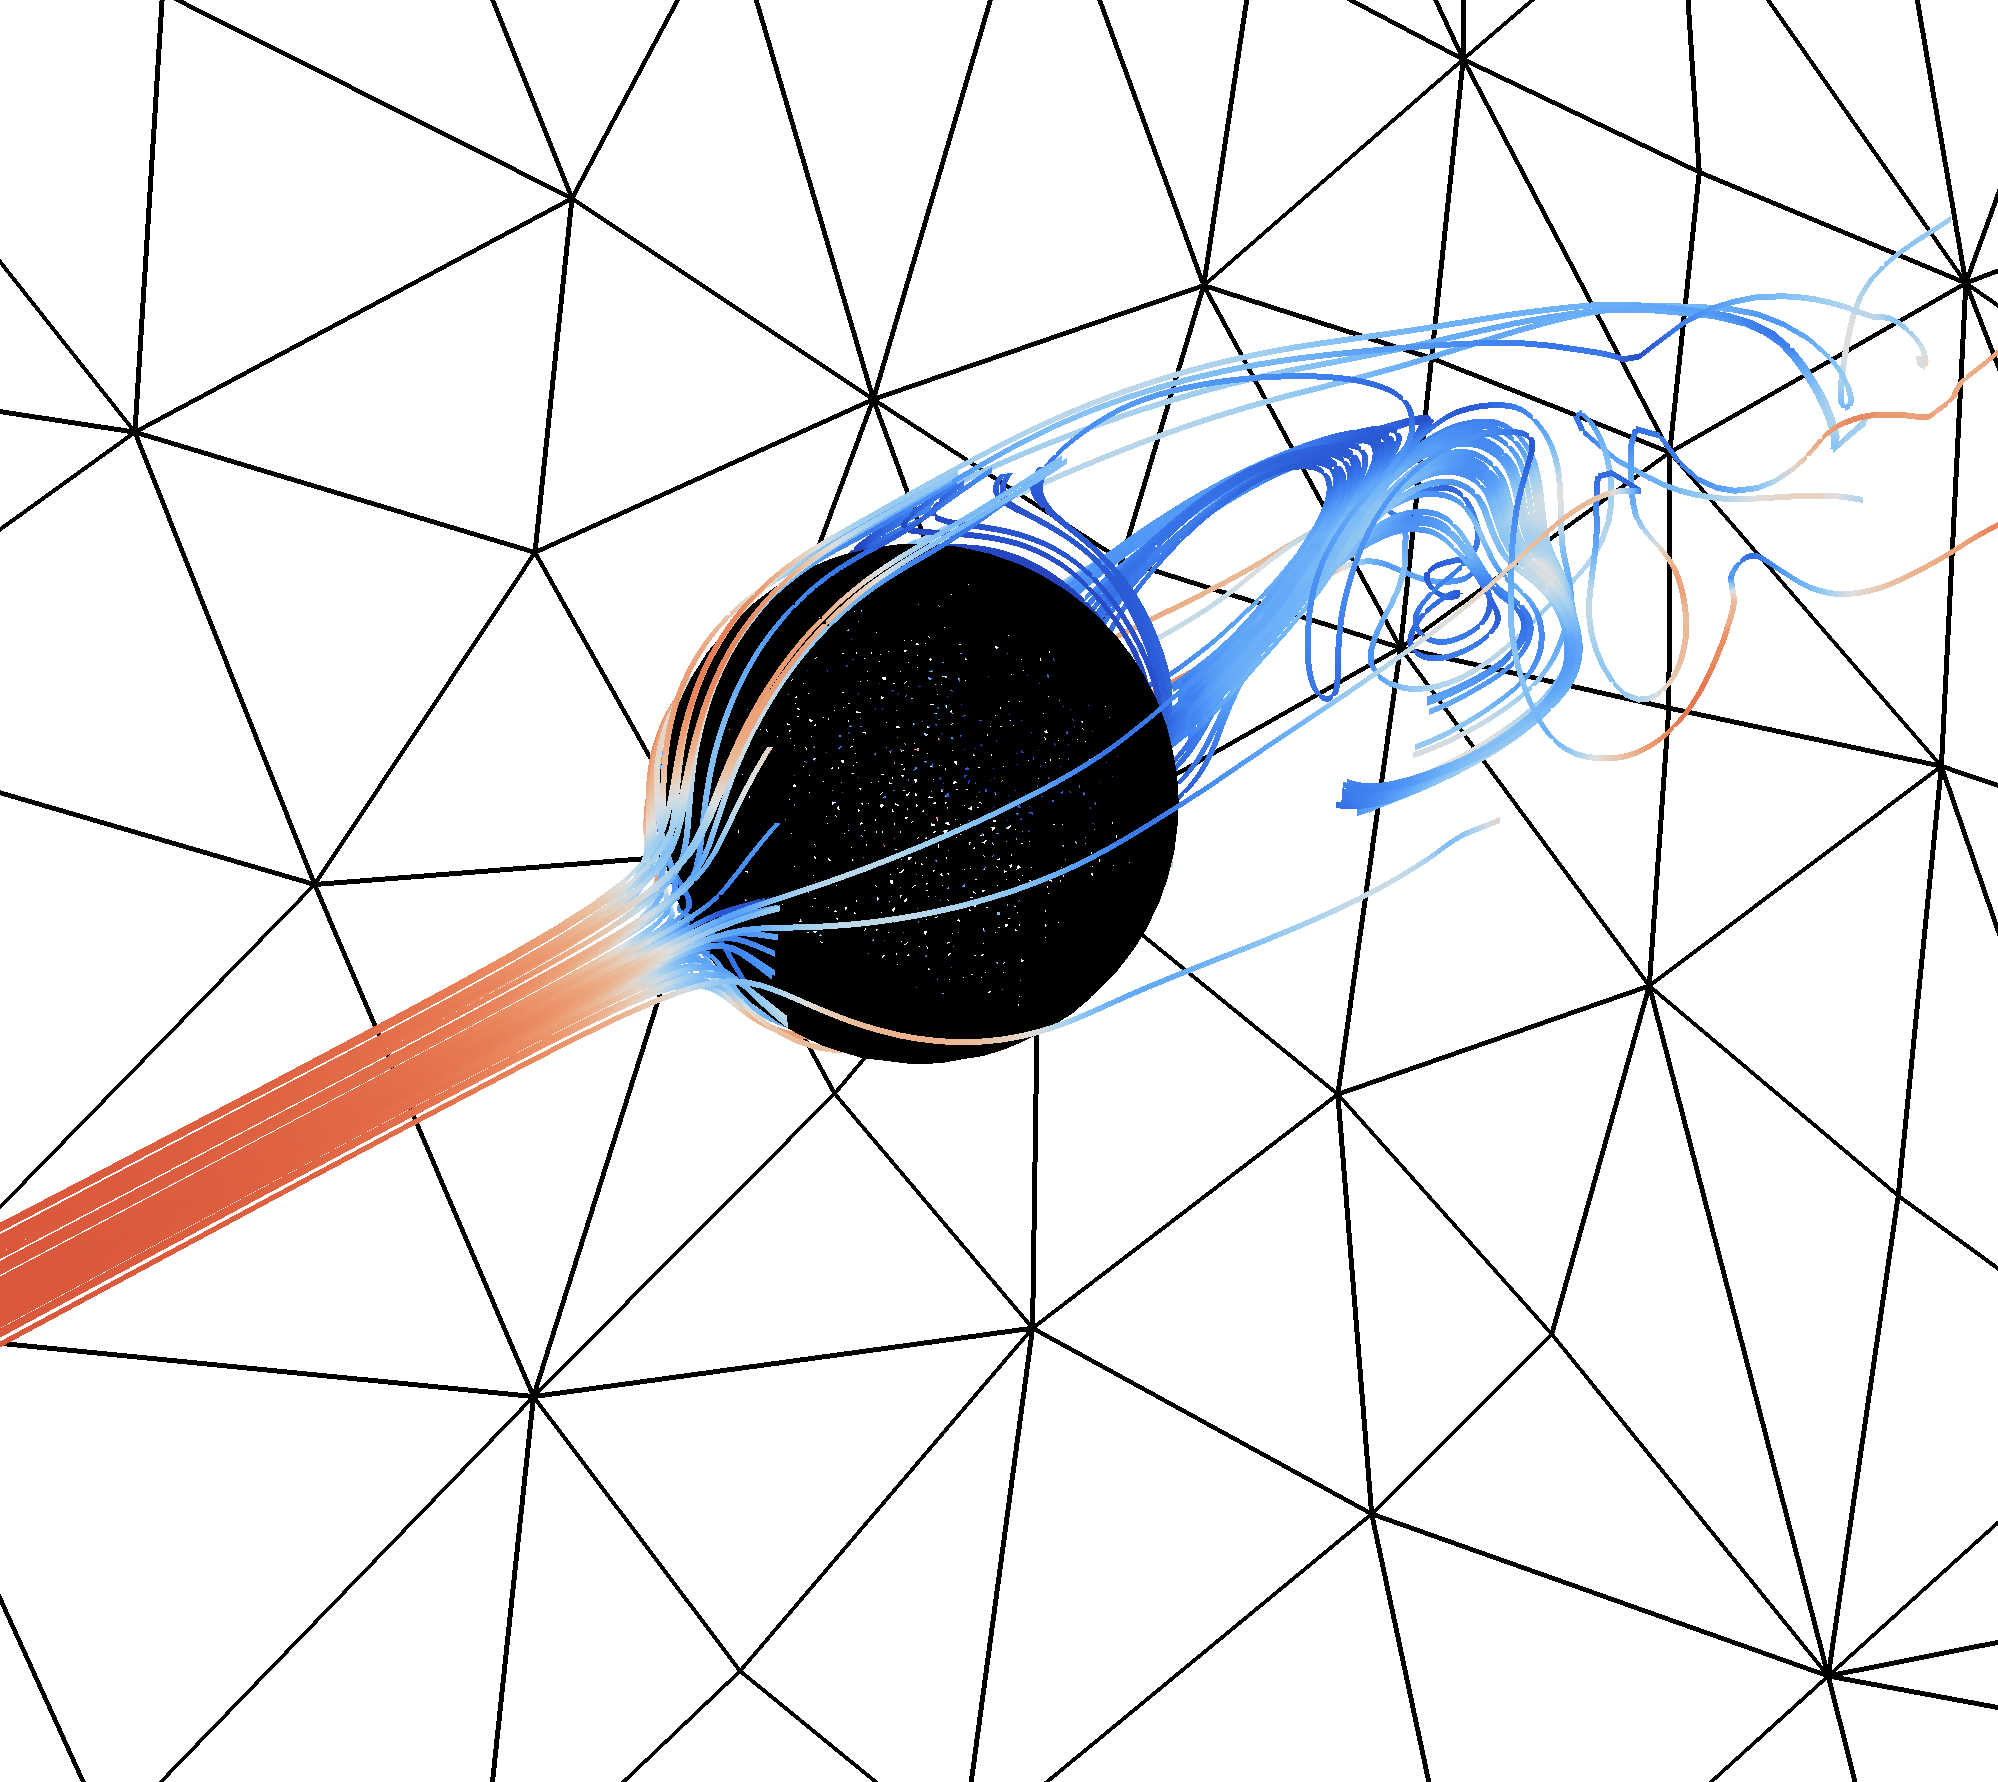
\includegraphics[width=0.225\textwidth]{./flow_past_sphere/sphere-Re1000-streamlines.png}}
\caption{Streamlines showing transition from laminar to turbulent wake with increasing Reynolds number.}
\end{figure}
\end{frame}

\begin{frame}
    \frametitle{Flow past a sphere}
\begin{figure}
\centering
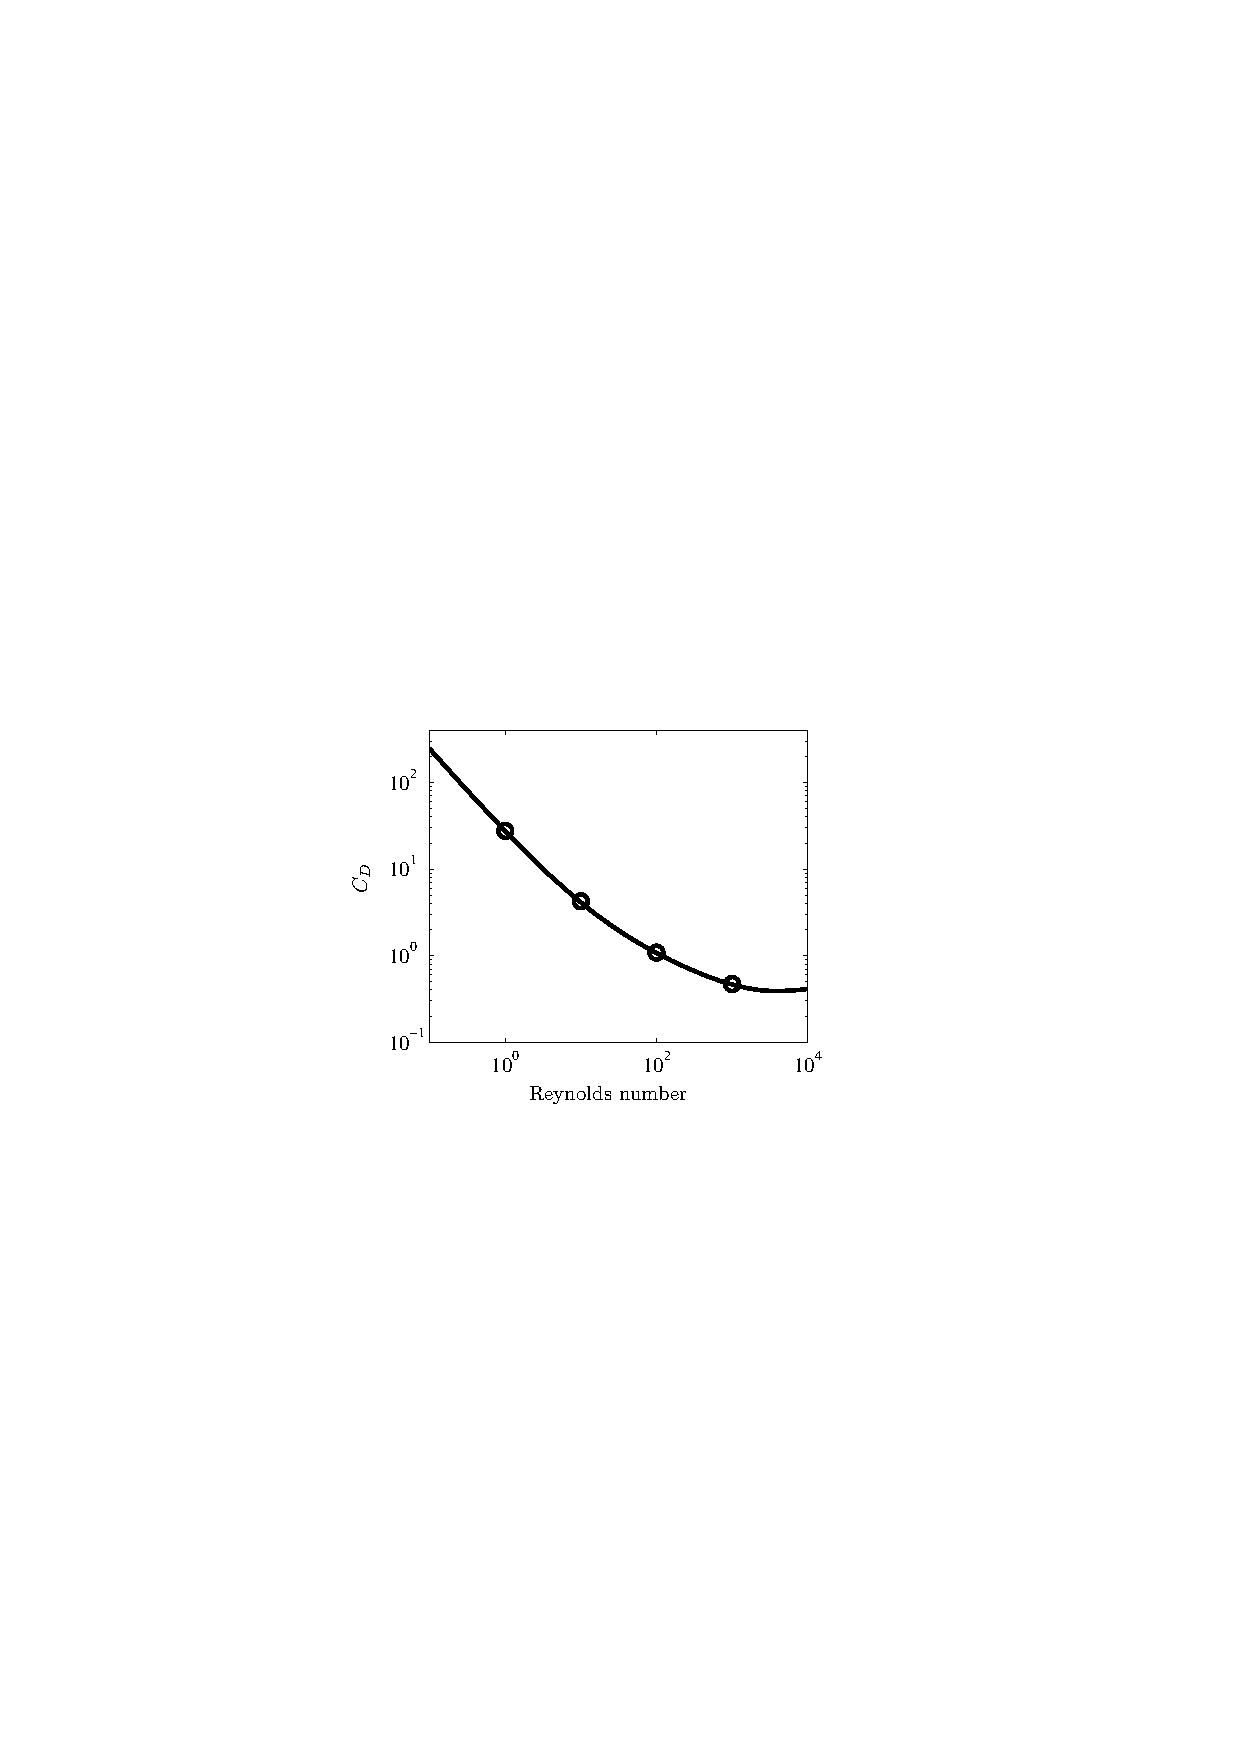
\includegraphics[width=0.5\textwidth]{./flow_past_sphere/Sphere_Drag.pdf}
\caption{Plot of drag coefficient vs. Reynolds number showing effect of turbulence. Circles: Fluidity data, line: correlation to experimental data from Brown and Lawler (2003), Journal of Environmental Engineering, 129(3).}
\end{figure}
\end{frame}

\begin{frame}
\frametitle{Flow past a sphere, exercises}
\begin{itemize}
\item Write an offline python diagnostic to calculate the drag.
\item Investigate impact different discretisations and adaptivity parameters on the drag.
\item Investigate different shaped objects.
\end{itemize}
\end{frame}

%-- Add sections and your outline will be created automatically --%
\subsection{Water collapse}

% Frame starts a new slide
\begin{frame}
    \frametitle{Water collapse}
\begin{itemize}
\item Multi--material problem: air, water
\item Compared to benchmark lab data
\item Barrier removed instantaneously at t = 0; flow driven by gravity
\end{itemize}

\begin{figure}
\centering
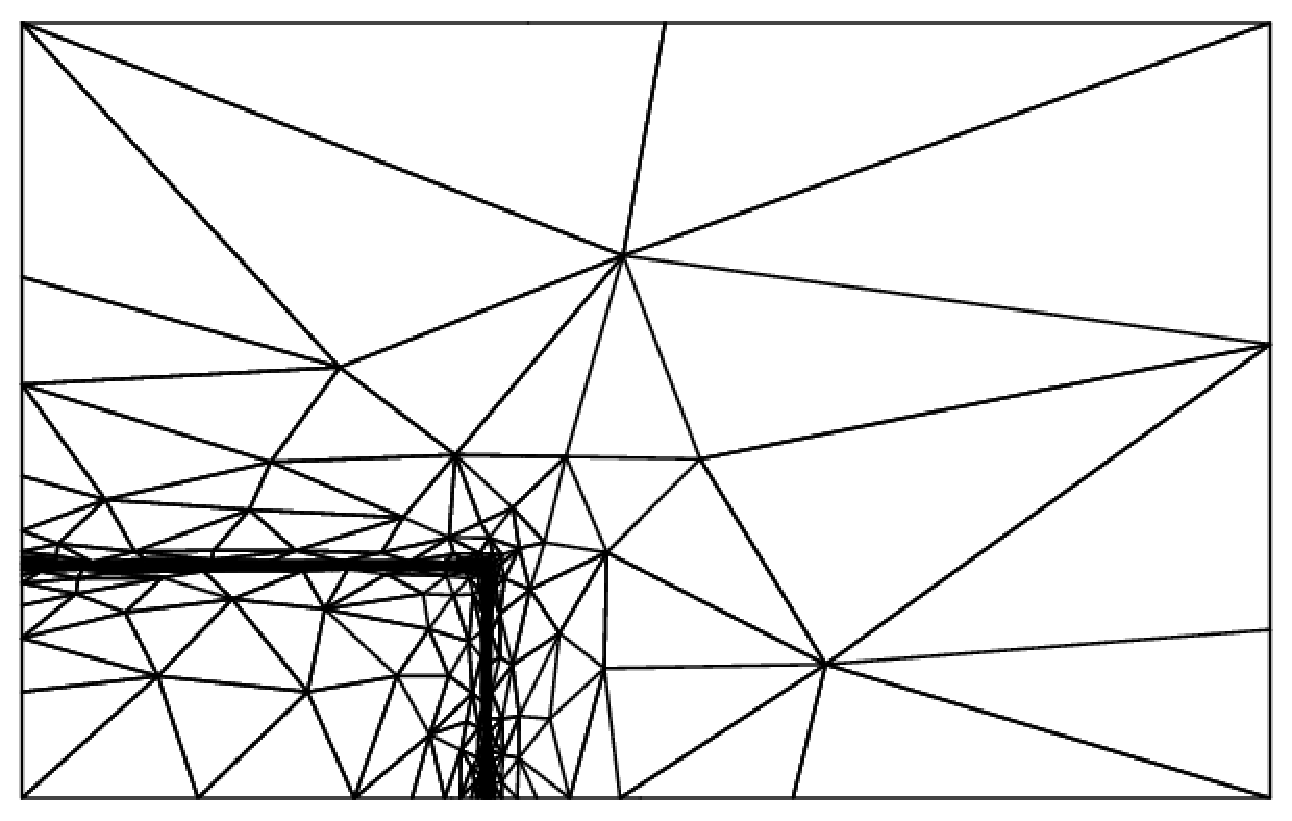
\includegraphics[width=0.6\textwidth, clip=true]{./water_collapse/water_collapse_0_mesh.pdf}
\caption{Initial unstructured adapted mesh for water collapse problem.}
\end{figure}

\end{frame}
%
\begin{frame}
    \frametitle{Water collapse}

\begin{figure}
\centering
\subfigure[$t=0.5$]{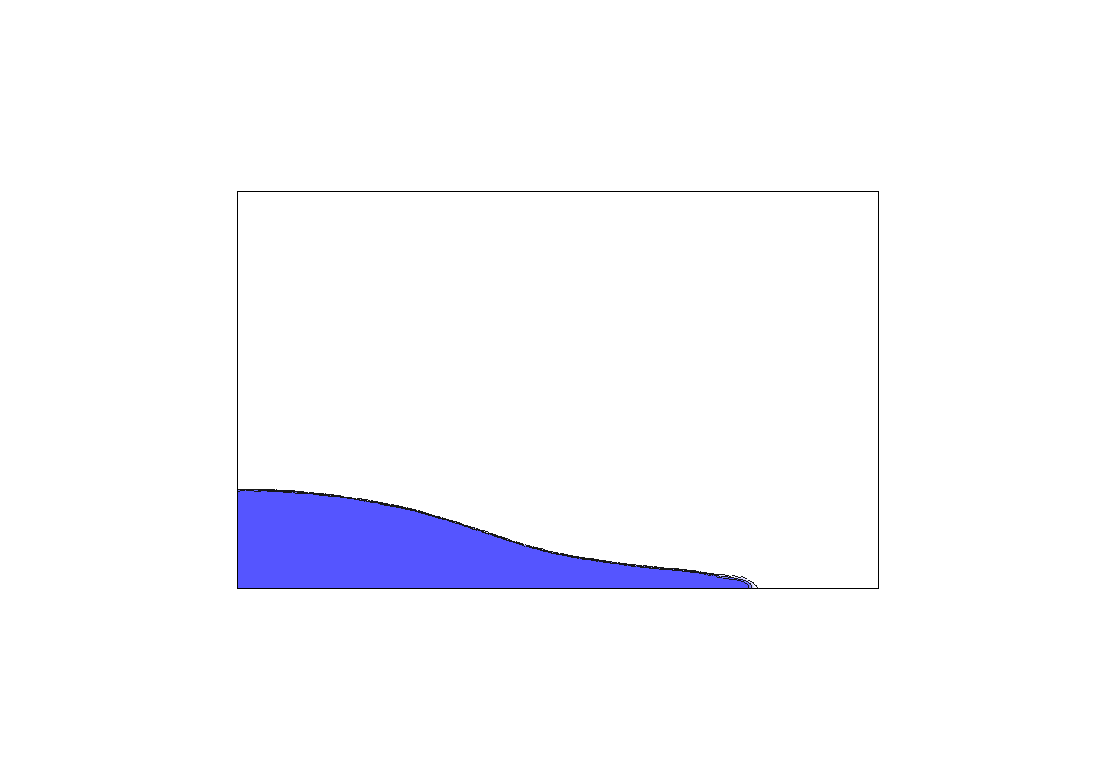
\includegraphics[width=0.275\textwidth, trim=7.5cm 6.5cm 7.5cm 6.5cm, clip=true]{./water_collapse/water_collapse_100.png}}
\subfigure[$t=1.0$]{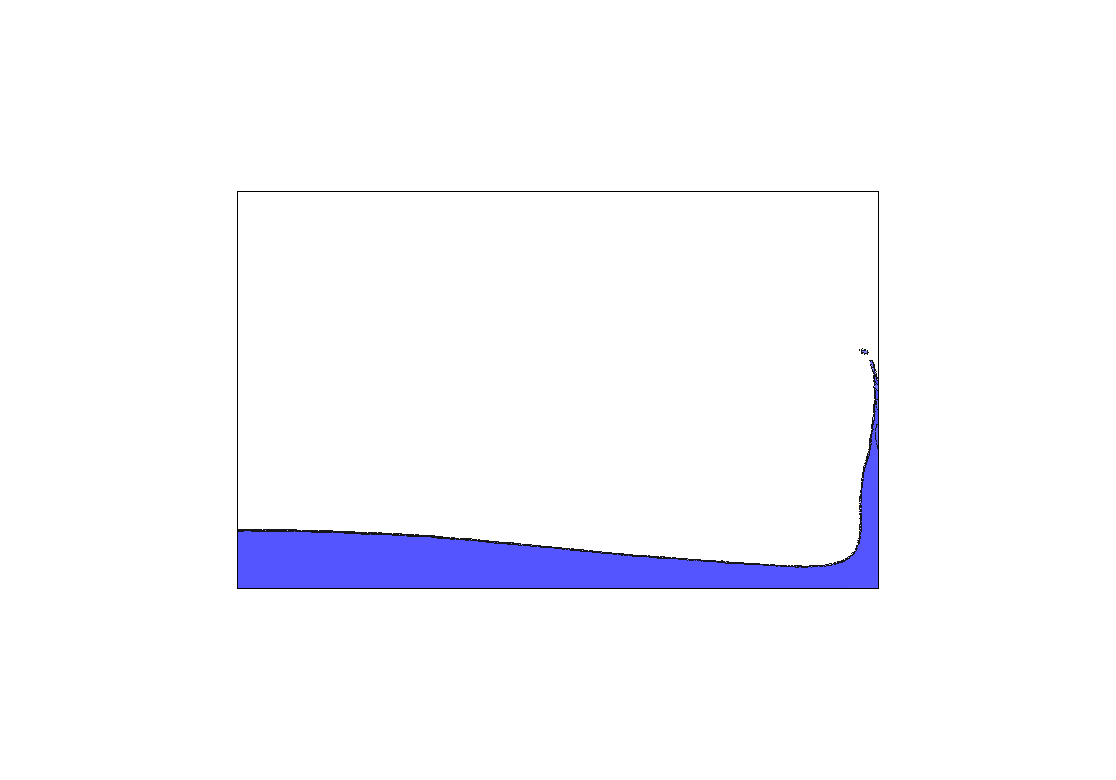
\includegraphics[width=0.275\textwidth, trim=7.5cm 6.5cm 7.5cm 6.5cm, clip=true]{./water_collapse/water_collapse_200.png}}
\subfigure[$t=1.5$]{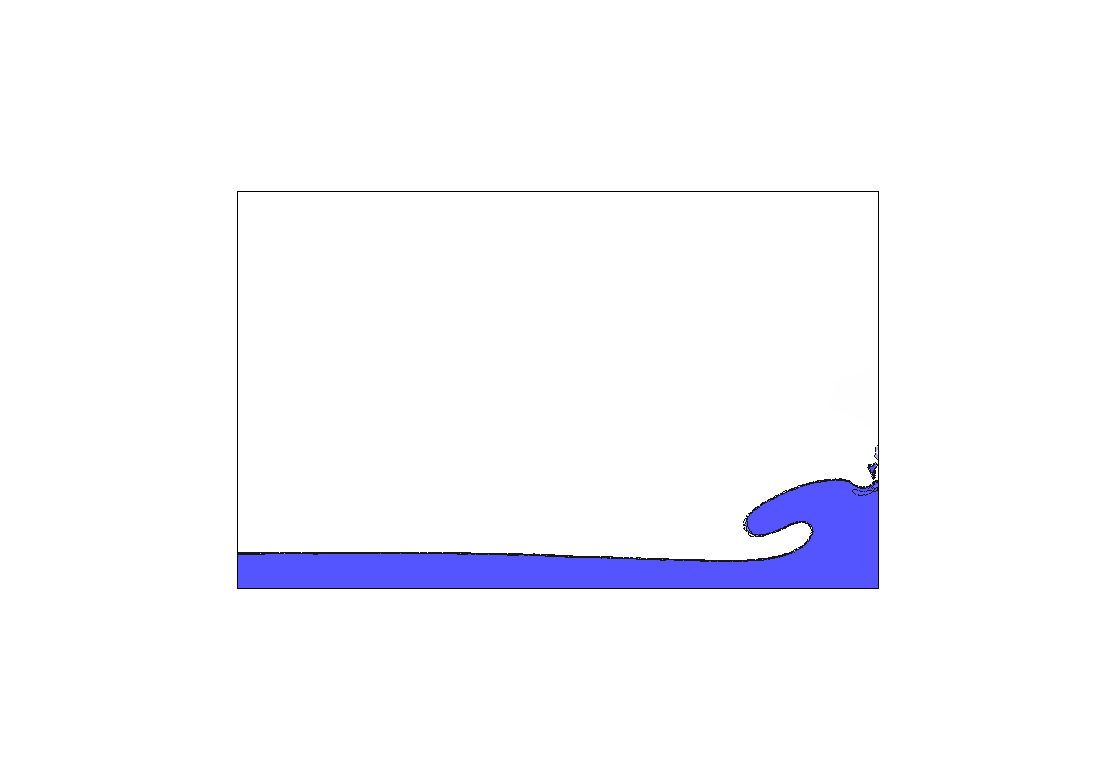
\includegraphics[width=0.275\textwidth, trim=7.5cm 6.5cm 7.5cm 6.5cm, clip=true]{./water_collapse/water_collapse_300.png}}
\subfigure[$t=1.75$]{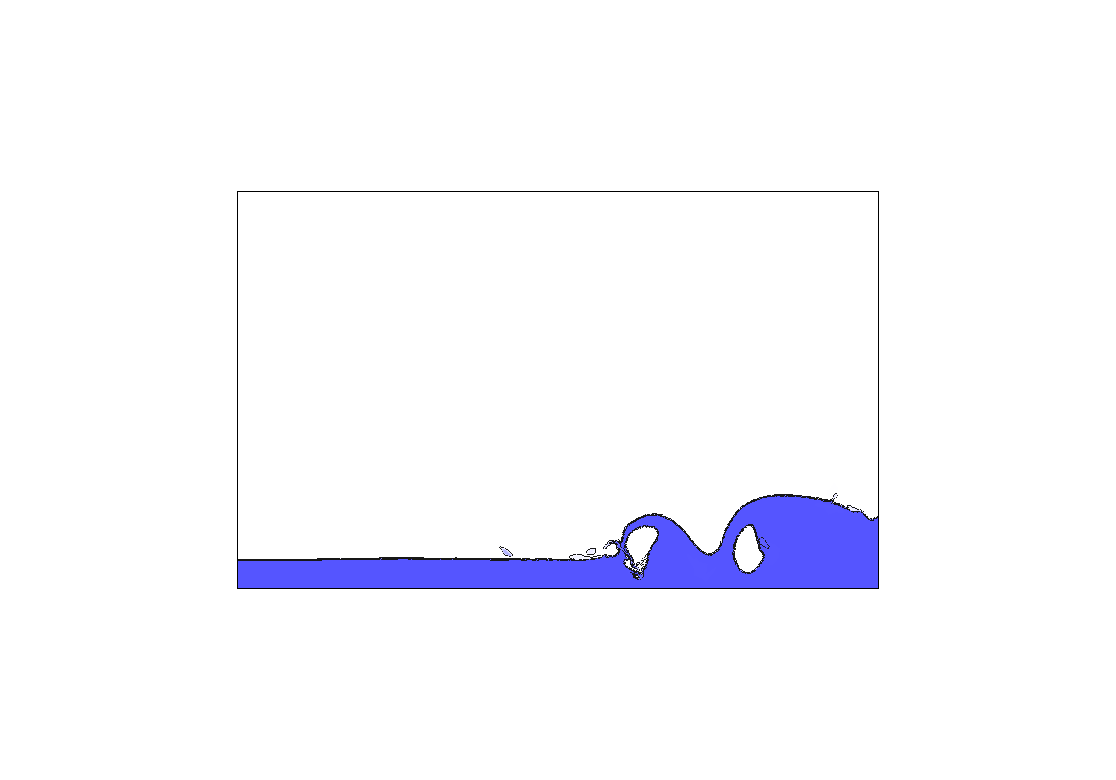
\includegraphics[width=0.275\textwidth, trim=7.5cm 6.5cm 7.5cm 6.5cm, clip=true]{./water_collapse/water_collapse_350.png}}
\subfigure[$t=2.25$]{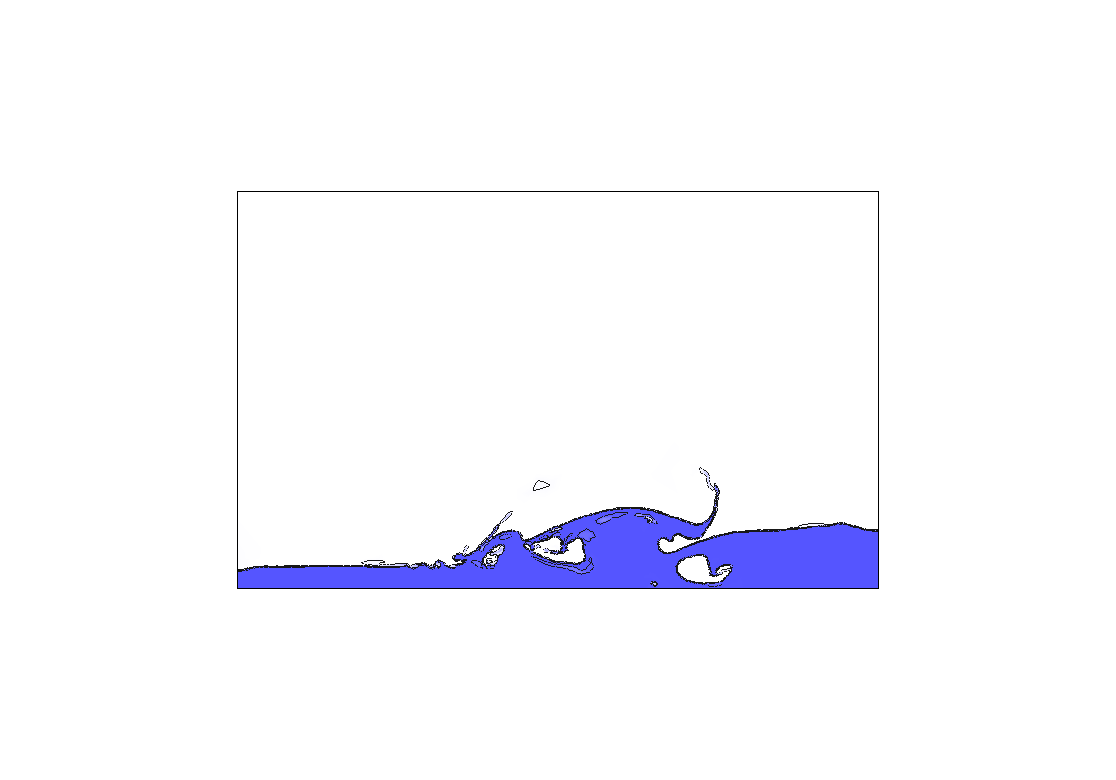
\includegraphics[width=0.275\textwidth, trim=7.5cm 6.5cm 7.5cm 6.5cm, clip=true]{./water_collapse/water_collapse_450.png}}
\subfigure[$t=2.5$]{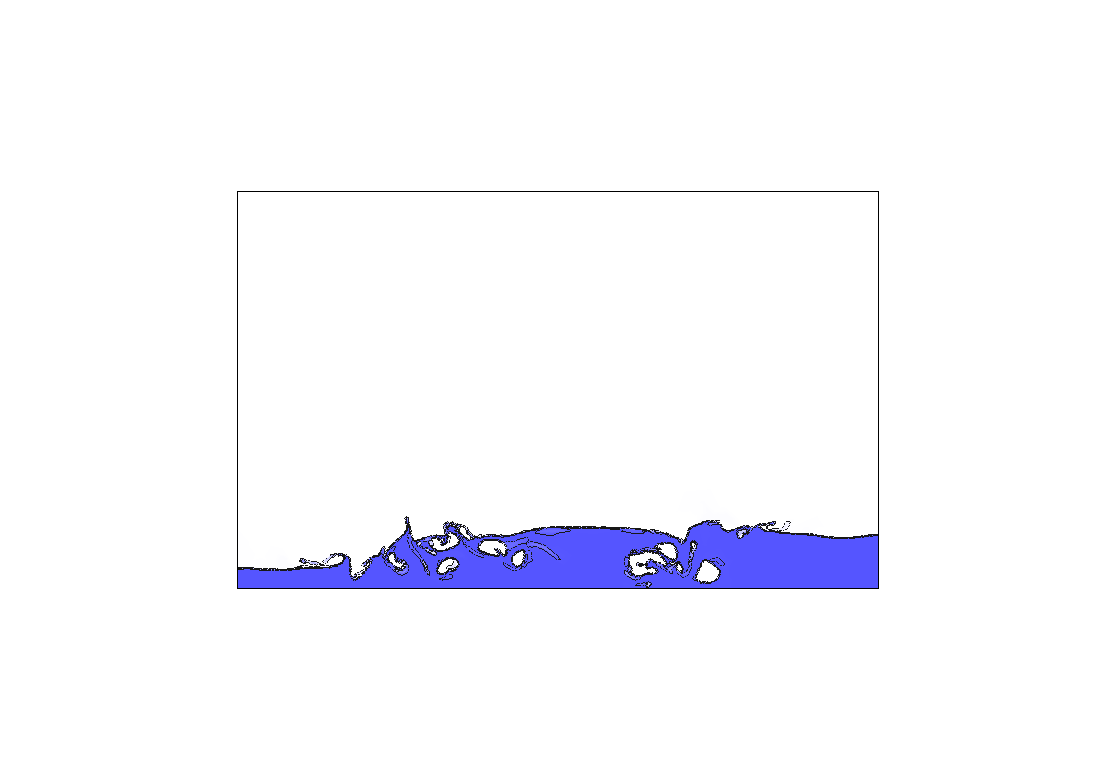
\includegraphics[width=0.275\textwidth, trim=7.5cm 6.5cm 7.5cm 6.5cm, clip=true]{./water_collapse/water_collapse_500.png}}
\caption{The evolution of the water volume fraction over several timesteps.  The presence of water is indicated as a blue region and the interface to the air is delineated by the contours (in black).}
\end{figure}

\end{frame}
%
\begin{frame}
    \frametitle{Water collapse}
\begin{itemize}
\item Post--processing scripts output several plots, e.g. comparison of water depth to experimental data
\end{itemize}
\begin{figure}
\centering
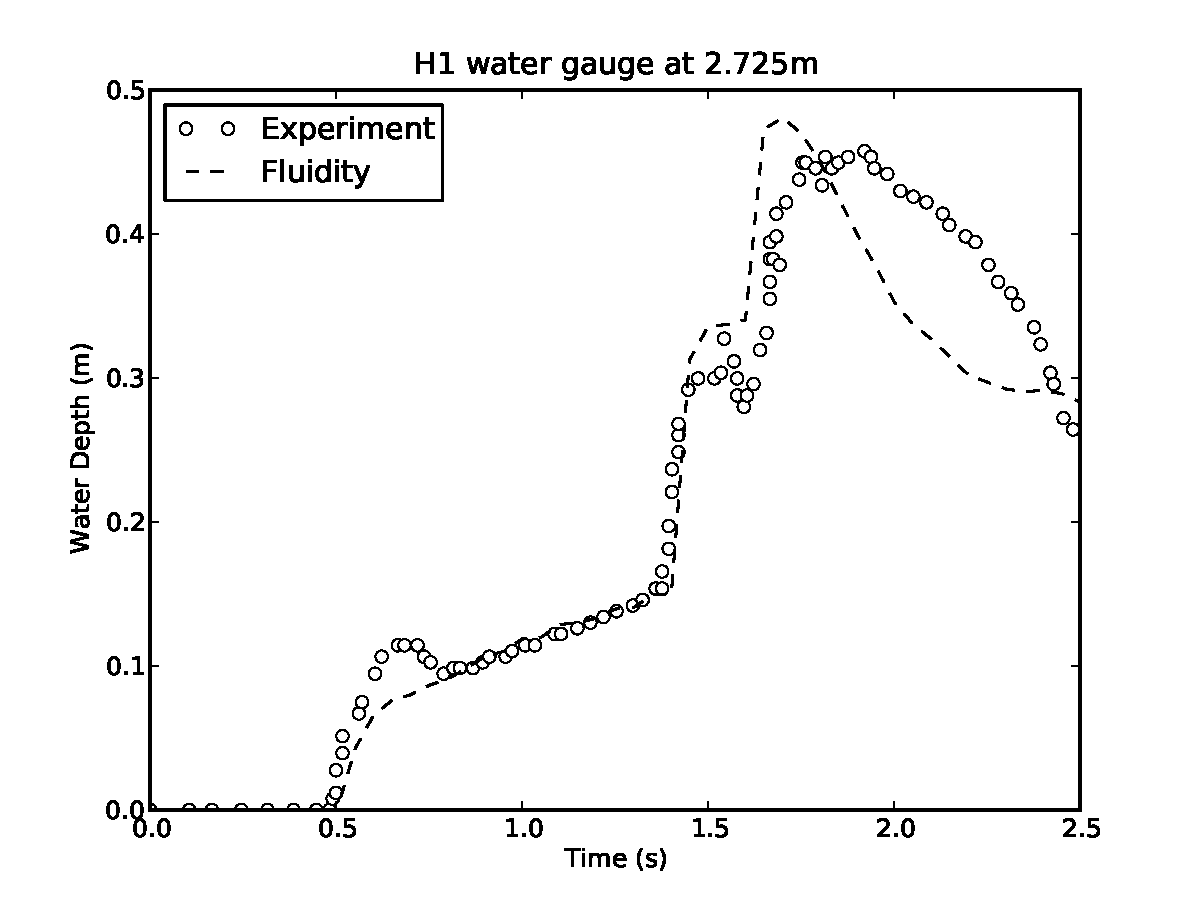
\includegraphics[width=0.5\textwidth]{./water_collapse/water_gauge_H1.pdf}
\caption{Comparison with experimental depth gauge data at $x = 2.725 \, $m.}
\end{figure}

\end{frame}
%
\begin{frame}
    \frametitle{Water collapse, exercises}
\begin{itemize}
\item Disable the adaptivity option to run on a fixed mesh.
\item Alter the water/air viscosity/density.
\item Modify the tank geometry.
\end{itemize}

\end{frame}

%-- Add sections and your outline will be created automatically --%
\subsection{Tephra settling}

% Frame starts a new slide
\begin{frame}
  \frametitle{Tephra settling}
  \begin{itemize}
  \item Replicates a laboratory experiment of tephra (fine volcanic ash particles) settling through a tank of water
    (Carey, 1997)
  \item Small tephra particles can settle either individually according to Stokes' law, or collectively as a cloud of particles (a plume)
  \item Dispersed multiphase approach, adaptive timestepping
  \item Run time: 1 hr.
    % \item Plumes are generated when the bulk density of the tephra-water mixture becomes large enough, yielding settling velocities much greater than those expected of single particles (which settle at a velocity given by Stokes law).
  \end{itemize}
\end{frame}

% \begin{frame}
%   \frametitle{Tephra settling - Simulation setup}
%   \begin{itemize}
%     \item The simulation uses a 0.3 x 0.7 metre domain, replicating the cross-section of the water tank used in the experiments.
%     \item No normal flow boundary conditions are weakly imposed along with a zero velocity initial condition, and the initial volume fraction of the particle phase is set to $1.0 \times 10^{-7}$.
%     \item The influx of particles from the air above is simulated using a \texttt{flux} boundary condition at the top of the domain. This allows tephra to flux in at a rate of $0.472\ \mathrm{gm^{-2}s^{-1}}$.
%   \end{itemize}
% \end{frame}

\begin{frame}
  \frametitle{Tephra settling - Numerical results (1)}
\begin{figure}[H]
        \centering
                
\includegraphics[scale=0.2]{tephra_settling/tephra_fine_1.png}\hspace{0.1cm}
                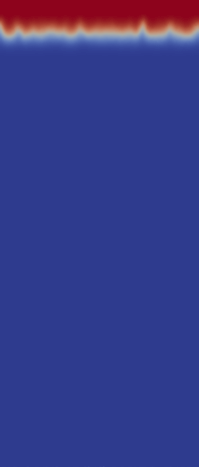
\includegraphics[scale=0.2]{tephra_settling/tephra_fine_2.png}\hspace{0.1cm}
                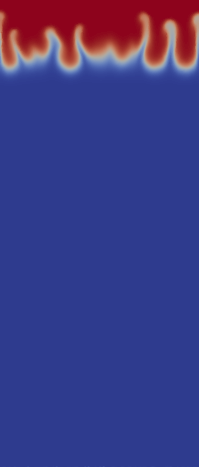
\includegraphics[scale=0.2]{tephra_settling/tephra_fine_3.png}\hspace{0.1cm}
                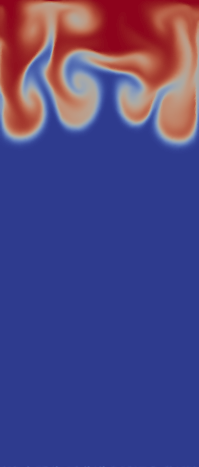
\includegraphics[scale=0.2]{tephra_settling/tephra_fine_4.png}\hspace{0.1cm}
                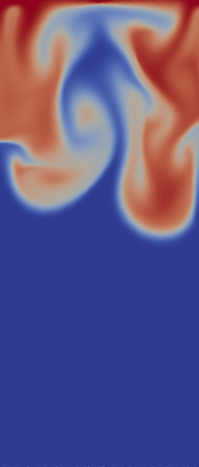
\includegraphics[scale=0.2]{tephra_settling/tephra_fine_5.png}
   \label{fig:tephra_adaptive}
   \caption{Simulation visualisations at $t = 10, 30, 50, 80$ and $110$ seconds. Tephra particles initially settle individually, but as more tephra fluxes in, the layer eventually becomes unstable and plumes begin to form.}
\end{figure}
\end{frame}

\begin{frame}
  \frametitle{Tephra settling - Numerical results (2)}
\begin{figure}[H]
        \centering
                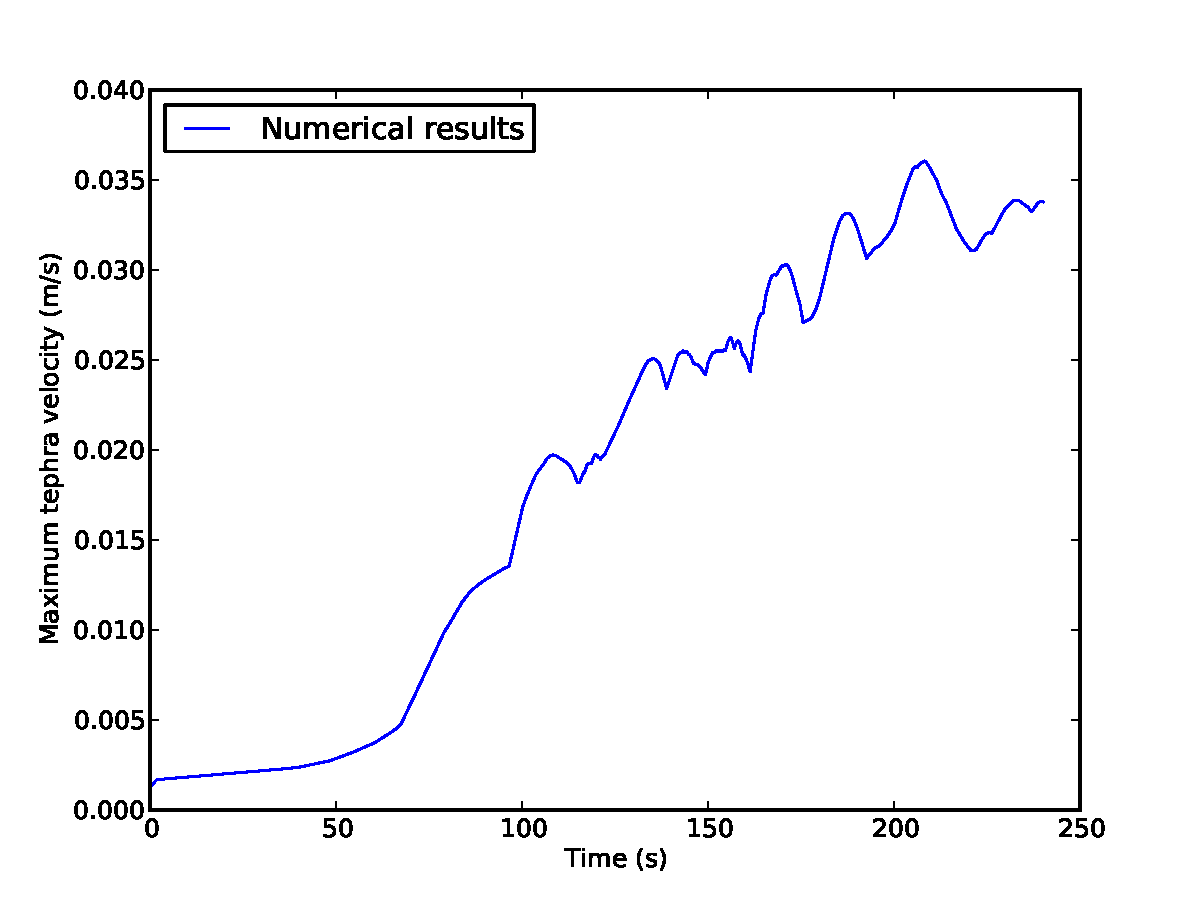
\includegraphics[scale=0.27]{tephra_settling/tephra_velocity.pdf}
   \label{fig:tephra_velocity}
   \caption{Plot of the maximum tephra phase velocity against time. Tephra particles initially settle at approximately $0.0017\ \mathrm{ms^{-1}}$, as predicted by Stokes' law. Plumes begin to form after approximately 30 seconds, resulting in settling velocities over 10 times greater than that of an individual particle.}
\end{figure}
\end{frame}

\begin{frame}
  \frametitle{Tephra settling - Exercises}
 \begin{itemize}
    \item Decrease the characteristic element size to better resolve the plume behaviour.\newline
    \item Alter the particle size to observe its effect on plume formation.\newline
    \item Add a second particle phase (with a different particle size).
 \end{itemize}
\end{frame}




\addtocontents{toc}{\newpage}

\section{GFD Examples}

%\documentclass[10pt]{beamer}
%\usetheme{amcg}
%\usepackage{subfigure}

%\begin{document}

\section{Lock--exchange}

\begin{frame}
  \frametitle{The lock--exchange}
  \begin{itemize}
  \item Flat bottomed tank, separated into two partitions by a barrier.
  \item Each half is filled with fluids of different density (temperature).
  \item The barrier is removed, and the denser fluid collapses under the lighter.
  \item The mesh changes in time as the dynamics evolves. 
  \end{itemize}

  \begin{figure}
    \centering
    
\includegraphics[width=0.45\textwidth]{./lock_exchange/le_basic_0_T}
    \caption{Lock-exchange initial temperature distribution.  Blue labels dense fluid, and red lighter.}
  \end{figure}
\end{frame}

\begin{frame}
  \frametitle{The lock--exchange}
  \begin{figure}[ht]
    \centering
    % For some reason tex4ht doesn't like these images.
    \subfigure[$t = 0\,$s]{
\includegraphics[width=0.45\textwidth]{./lock_exchange/le_basic_0_T}}
    \subfigure[$t = 0\,$s]{\includegraphics[width=0.45\textwidth]{./lock_exchange/le_basic_0_mesh_nice}} \\
    \subfigure[$t = 12.475\,$s]{
\includegraphics[width=0.45\textwidth]{./lock_exchange/le_basic_10_T}}
    \subfigure[$t = 12.475\,$s]{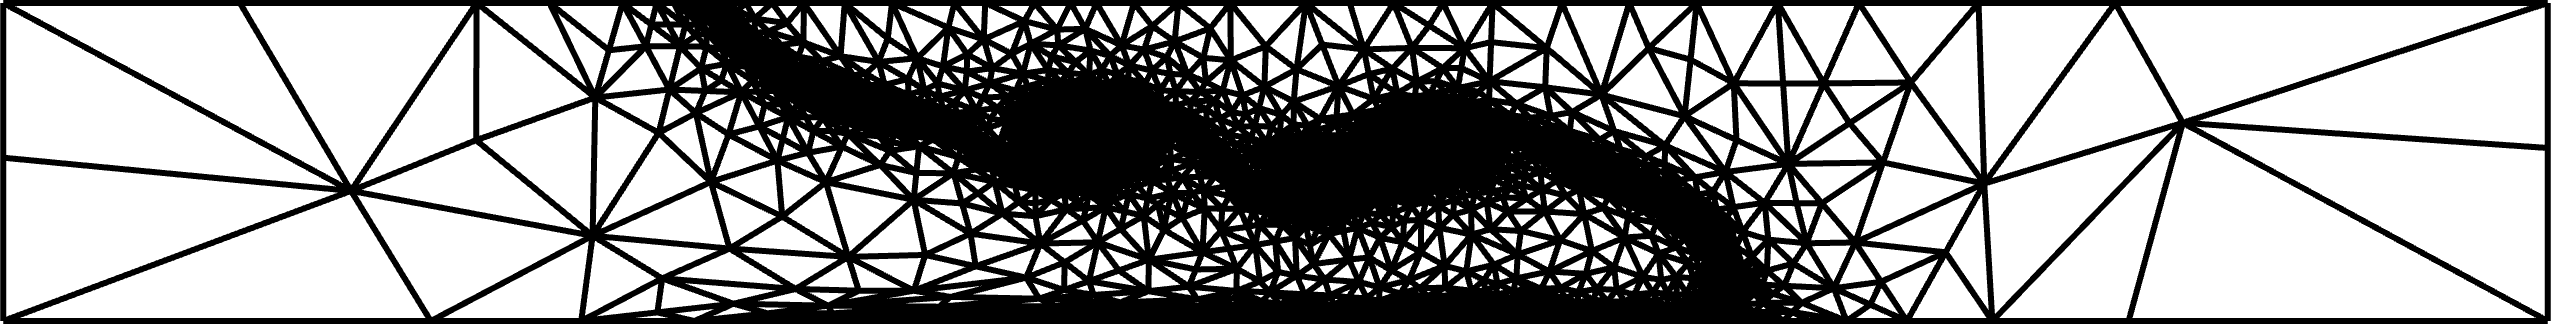
\includegraphics[width=0.45\textwidth]{./lock_exchange/le_basic_10_mesh}} \\
    \subfigure[$t = 37.475\,$s]{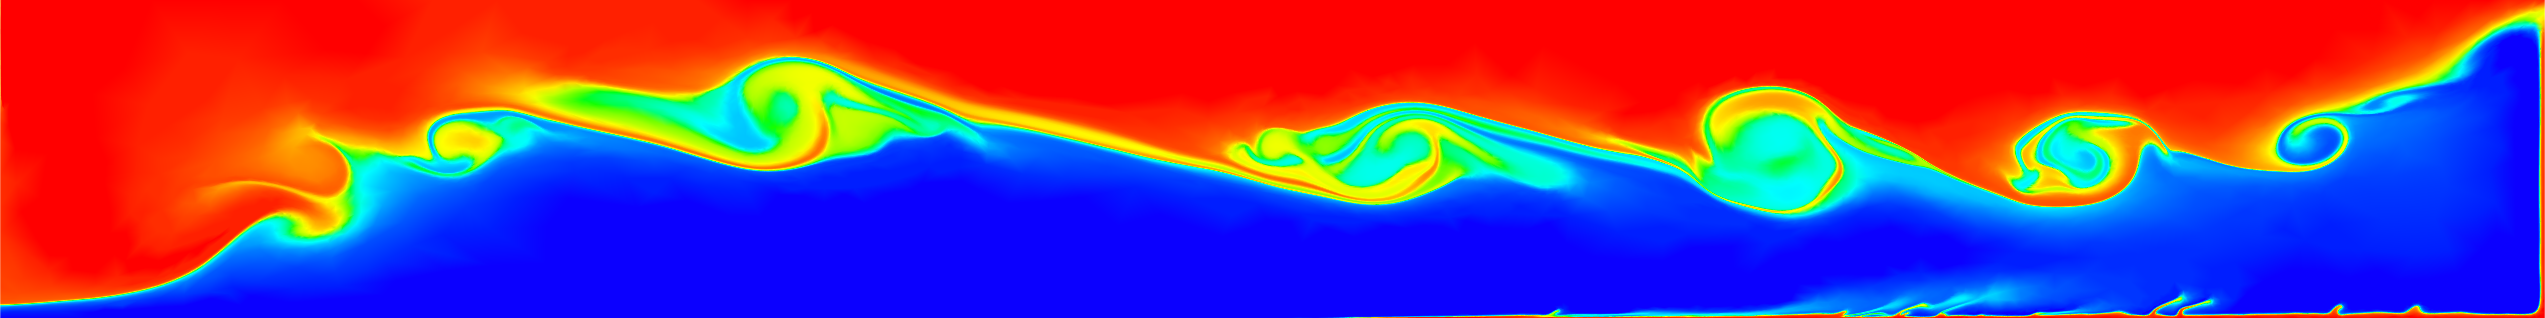
\includegraphics[width=0.45\textwidth]{./lock_exchange/le_basic_30_T}}
    \subfigure[$t = 37.475\,$s]{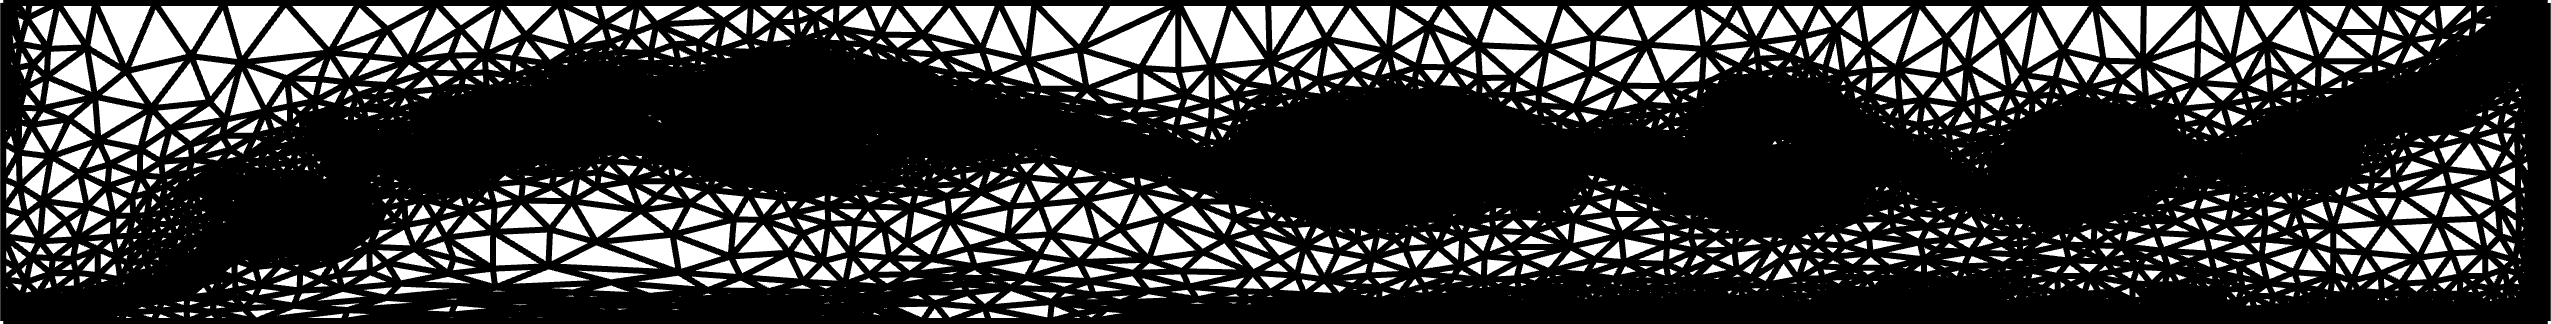
\includegraphics[width=0.45\textwidth]{./lock_exchange/le_basic_30_mesh}}
    \caption{Lock-exchange temperature distribution (colour) with meshes, over time ($t$).}
  \end{figure}
\end{frame}
 
\begin{frame}
  \frametitle{The lock--exchange, diagnostics}
  \begin{itemize}
  \item Front speed (or Froude number).
  \item Mixing indicated by domain fractions of fluid in specified temperature classes.
  \end{itemize}

  \begin{figure}
    \centering
    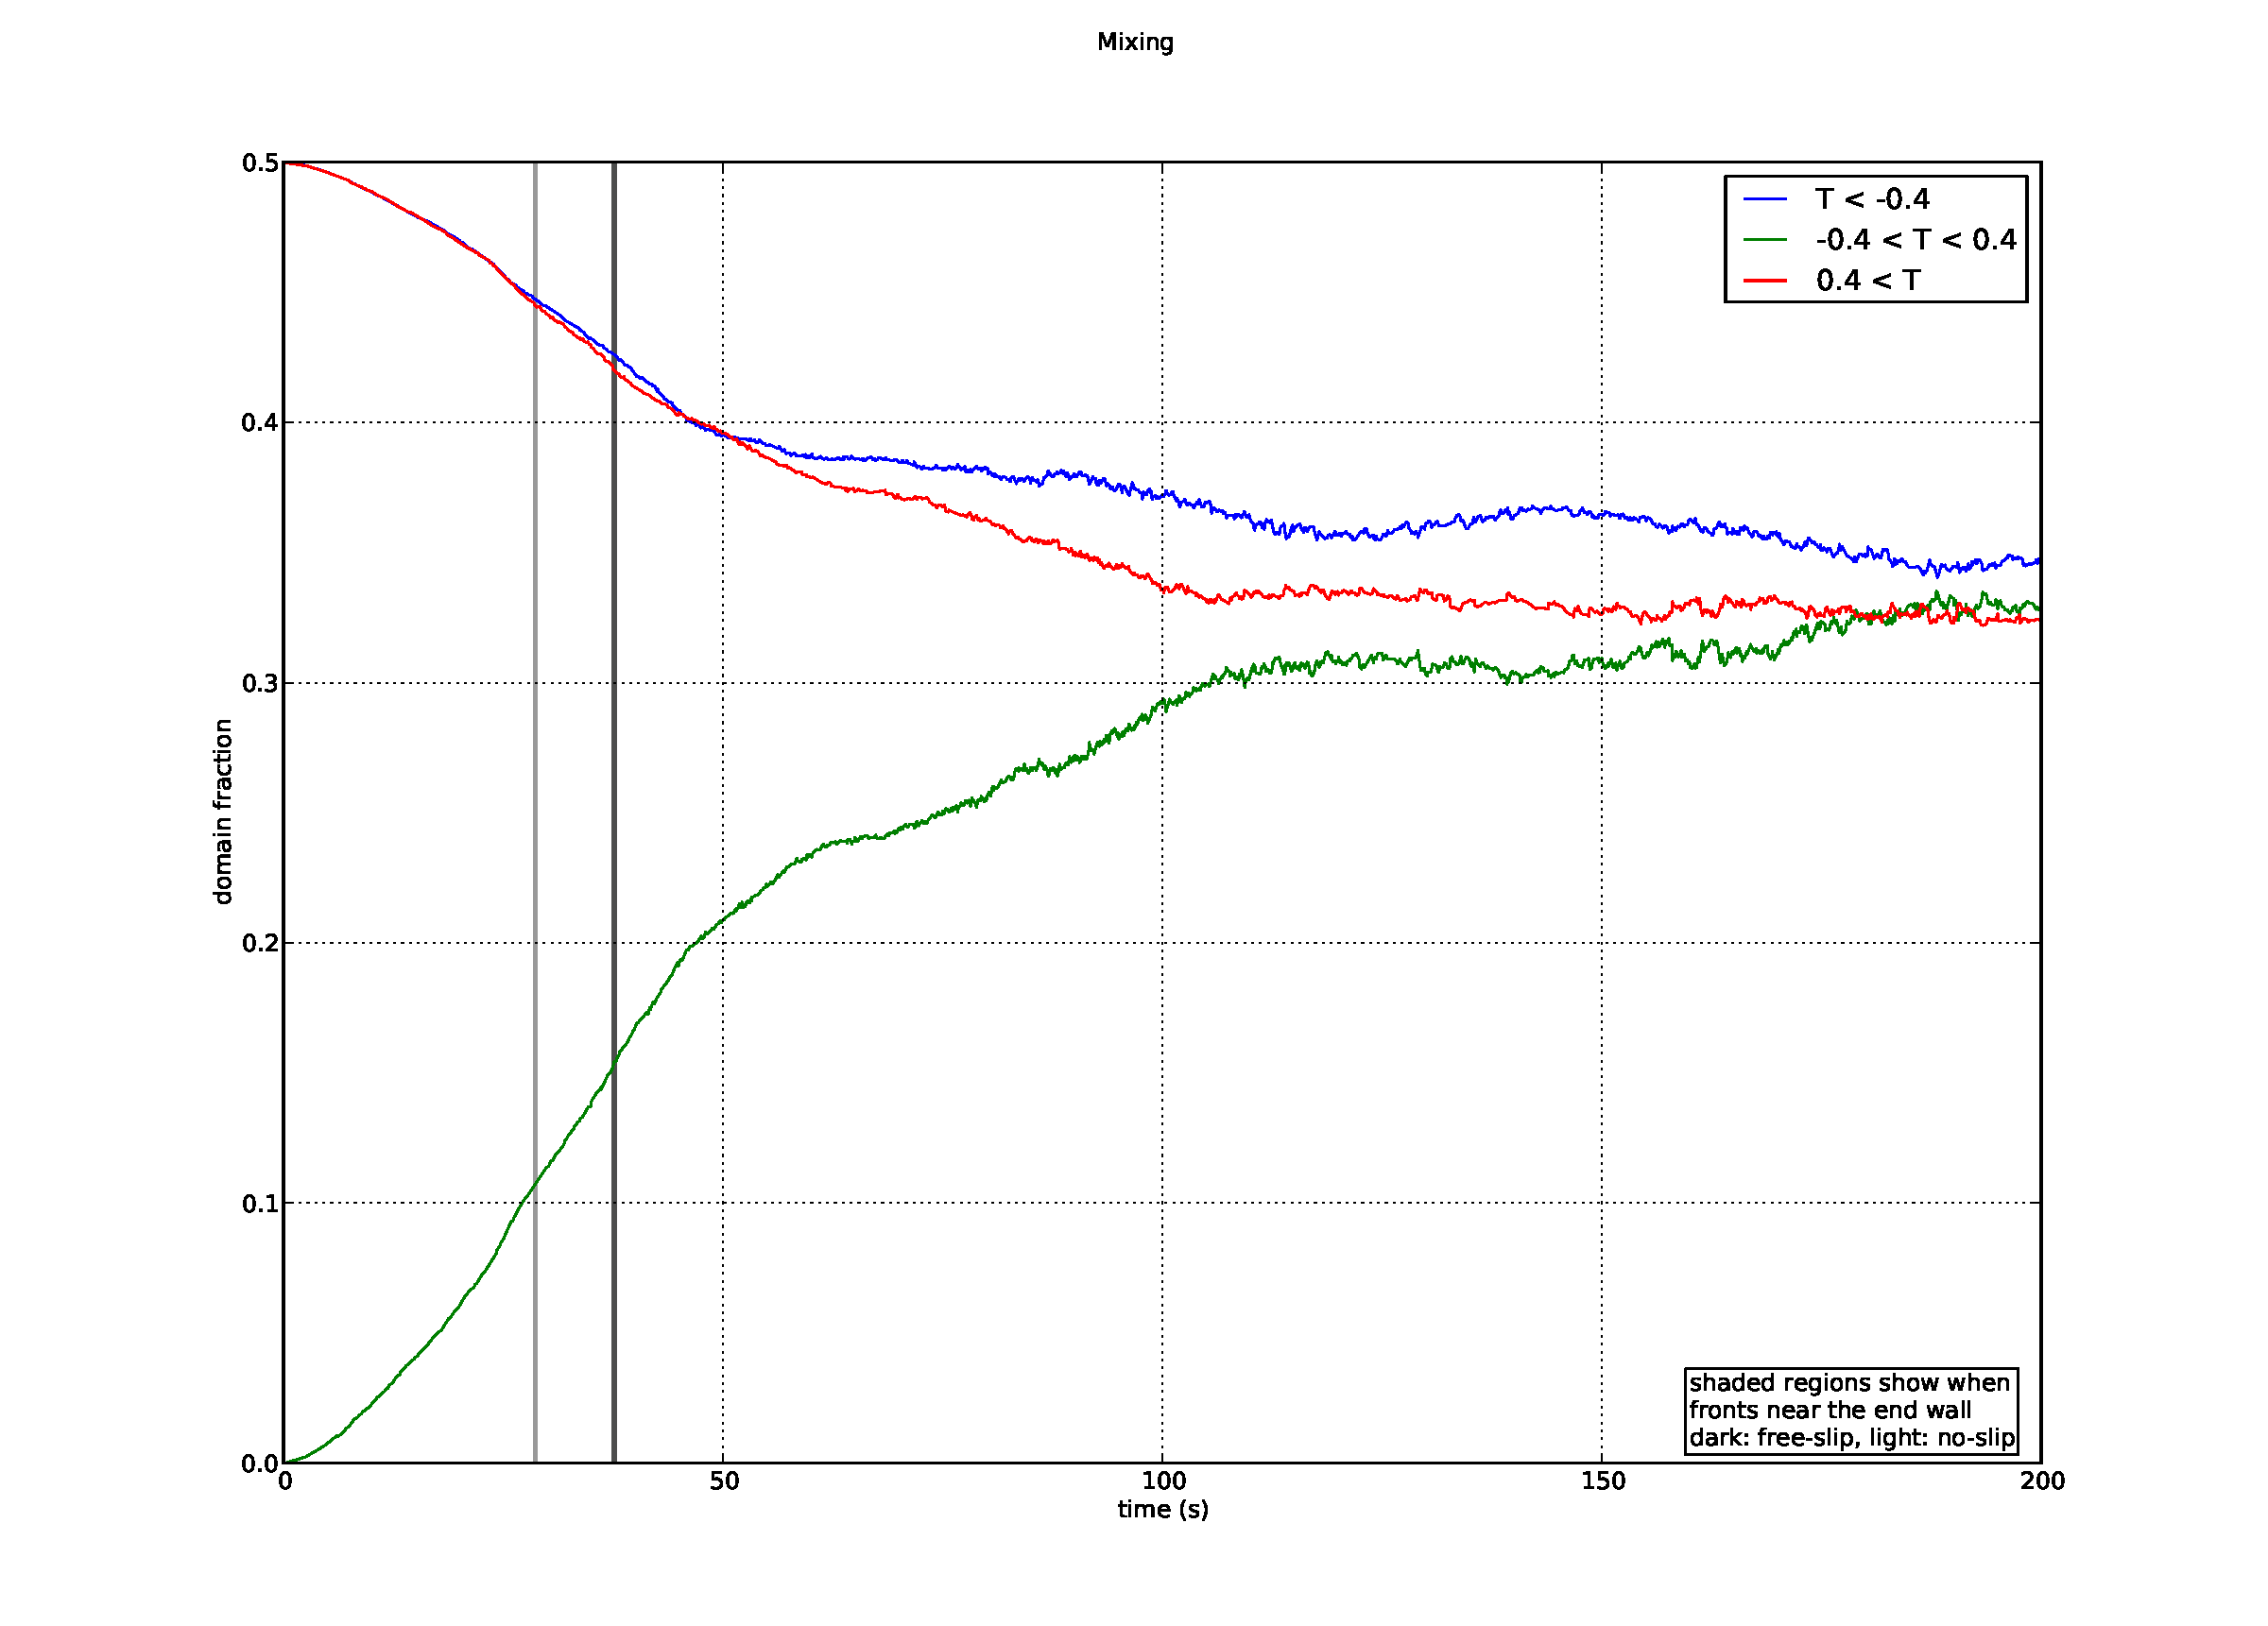
\includegraphics[width=0.5\textwidth]{./lock_exchange/mixing}
    \caption{Time evolution of fraction of domain that contains fluid in three temperature classes. Blue: cold, red: warm, green: mixed}
  \end{figure}
\end{frame} 

\begin{frame}
  \frametitle{The lock--exchange, exercises}
  \begin{itemize}
  \item Experiment with the adaptivity options.
  \item Try adding some detectors to visualise the particle trajectories.
  \end{itemize}
\end{frame}

%\end{document}

%-- Add sections and your outline will be created automatically --%
\section{Tsunami}

% Frame starts a new slide
\begin{frame}
    \frametitle{Hokkaido-Nansei-Oki tsunami}
\begin{minipage}[]{0.5\linewidth} 
\begin{itemize}
\item Okushiri island, Japan, 1993. 
\item Runup height of up to 30m.
\item Simulation based on a 1:400 laboratory setup.
\item Uses the free-surface and wetting and drying functionality of Fluidity.
\end{itemize}
\end{minipage}
\hspace{0.5cm}
\begin{minipage}[]{0.4\linewidth} 
\begin{figure}
\begin{center}
\includegraphics[width=\textwidth]{hokkaido-nansei-oki_tsunami/MonaiValleyDomainWithInputWave2_png.pdf}
\end{center}
\caption{The domain and the three gauge stations.}\label{fig:monai_inputwave}
\end{figure}
\end{minipage}
\end{frame}

\begin{frame}
    \frametitle{Hokkaido-Nansei-Oki tsunami}
\begin{figure}
\begin{center}
\includegraphics[width=0.7\textwidth]{hokkaido-nansei-oki_tsunami/MonaiValley_C_p1p1_nu0_01_kmkstab_drag0_002_butcircularoundisland0_2-crop-crop_final2.pdf}
\caption{The numerical and experimental results at the three gauge stations.}\label{fig:monai_results}
\end{center}
\end{figure}
% end my slide
\end{frame}


\begin{frame}
    \frametitle{Hokkaido-Nansei-Oki tsunami - Exercises}
  \begin{itemize}
    \item Add more detectors.\newline
    \item Check how increasing the wetting and drying threshold parameter affects the results.\newline
    \item Try changing the viscosity value (How does it affect the inundation of the tsunami event?).
  \end{itemize}
% end my slide
\end{frame}



%-- Add sections and your outline will be created automatically --%
\section{Rotating periodic channel}

% Frame starts a new slide
\begin{frame}
    \frametitle{Rotating periodic channel}
\begin{itemize}
\item Domain: Unit square, periodic in zonal direction.
\item Boundary conditions: No-slip at the North and South boundaries.
\item Coriolis applied.
\item Forcing applied by a Python function.
\item The flow is driven by a velocity source term:
\begin{equation*}
  \vec{F}=
  \begin{bmatrix}
    y^3 \\
    0
  \end{bmatrix}
\end{equation*}
\item Parameters are chosen such that the solution converges to a steady state with a known analytical solution.
\end{itemize}
\end{frame}
%
\begin{frame}
    \frametitle{Rotating periodic channel}
\begin{figure}
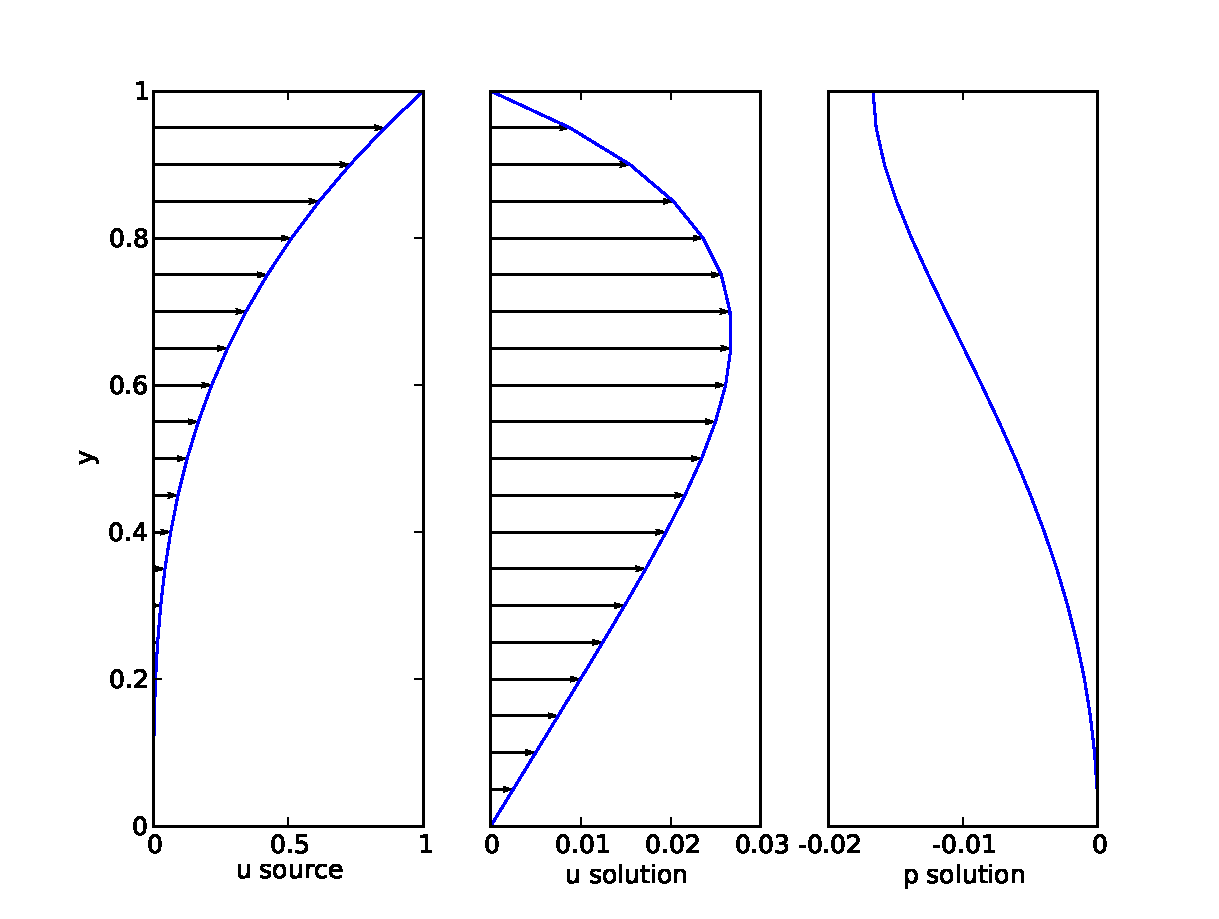
\includegraphics[width=0.6\textwidth]{./rotating_channel/analytic_solution}
\caption{Velocity forcing term and analytic solutions for velocity and pressure.  Each of these quantities are constant in the x direction.}
\end{figure}
\end{frame}
%
\begin{frame}
    \frametitle{Rotating periodic channel}
\begin{figure}
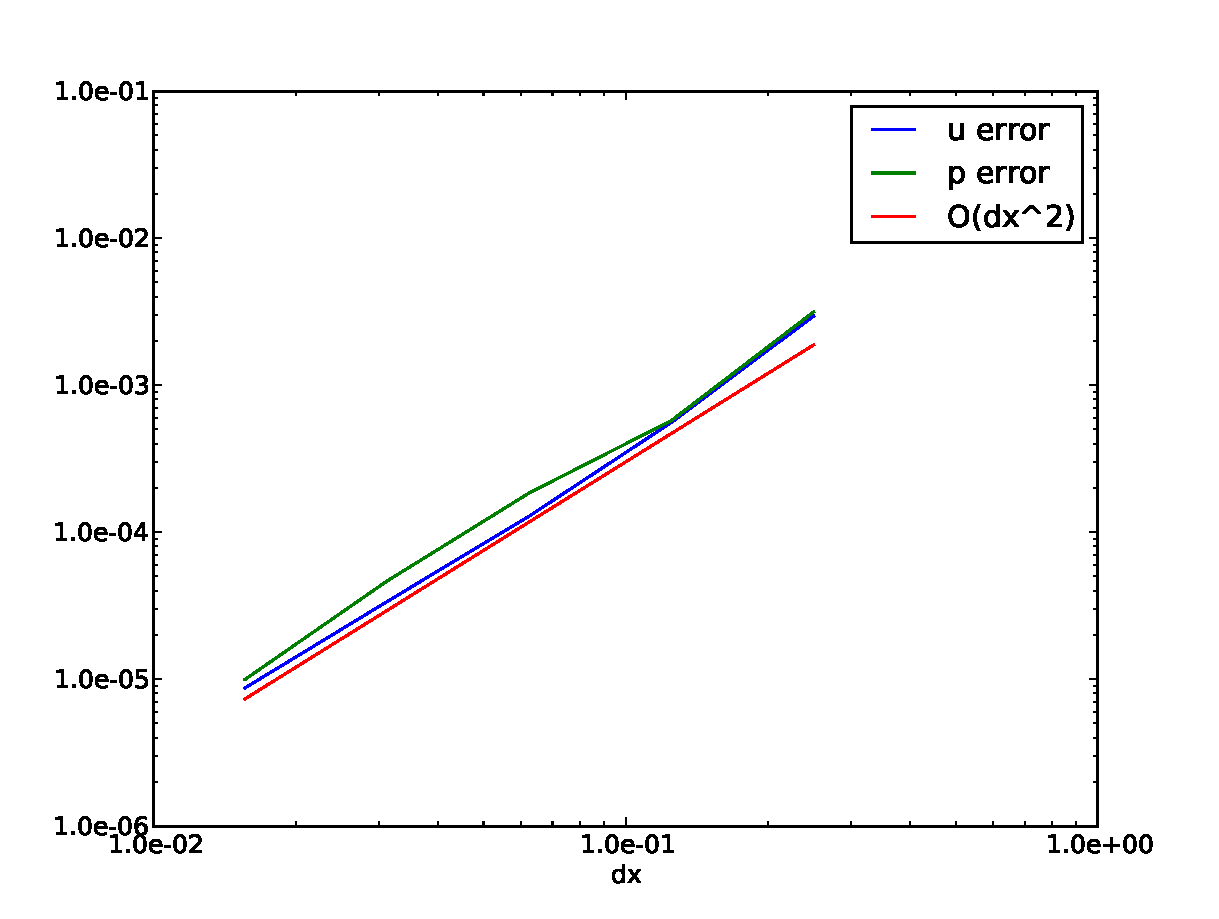
\includegraphics[width=0.6\textwidth]{./rotating_channel/convergence}
\caption{Error in the pressure and velocity solutions as a function of mesh resolution.}
\end{figure}
\end{frame}
%
\begin{frame}
    \frametitle{Rotating periodic channel, exercises}
\begin{itemize}
\item Understand the use of analytic forcing functions in Fluidity using Python (e.g. take a look at \url{channel_tools.py} and \url{plot_theory}).
\end{itemize}
\end{frame}


%-- Add sections and your outline will be created automatically --%
\section{Restratification following open ocean deep convection}

% Frame starts a new slide
\begin{frame}
    \frametitle{Restratification following open ocean deep convection}
\begin{itemize}
\item Idealised model of the restratification phase of OODC using $P_1DGP_2$ using an extruded mesh.
\end{itemize}
\begin{figure}
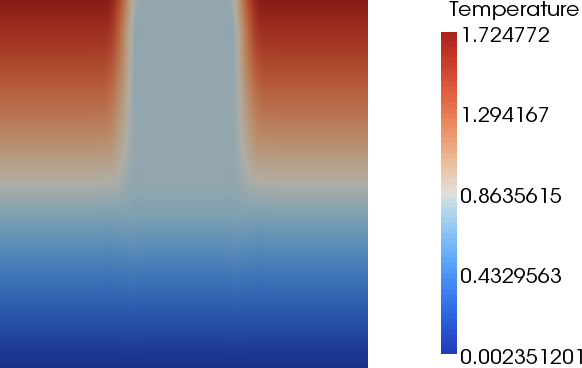
\includegraphics[width=0.5\textwidth]{./restratification_after_oodc/rousset-init.png}
\caption{A vertical slice throughout the domain showing the initial temperature stratification. The domain is a cylinder of radius $250 \,$km and height $1\,$km.}
\end{figure}
\end{frame}
%
\begin{frame}
    \frametitle{Restratification following open ocean deep convection}
\begin{figure}
\centering
\subfigure [0 days]{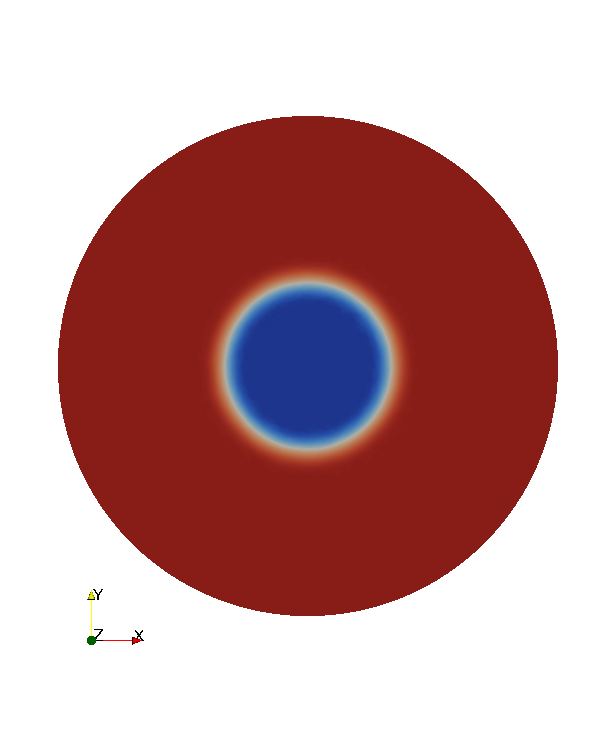
\includegraphics[width=0.175\textwidth]{./restratification_after_oodc/rousset-res5000-depth-40m0001.png}}
\subfigure [10 days]{
\includegraphics[width=0.175\textwidth]{./restratification_after_oodc/rousset-res5000-depth-40m0003.png}}
\subfigure [20 days]{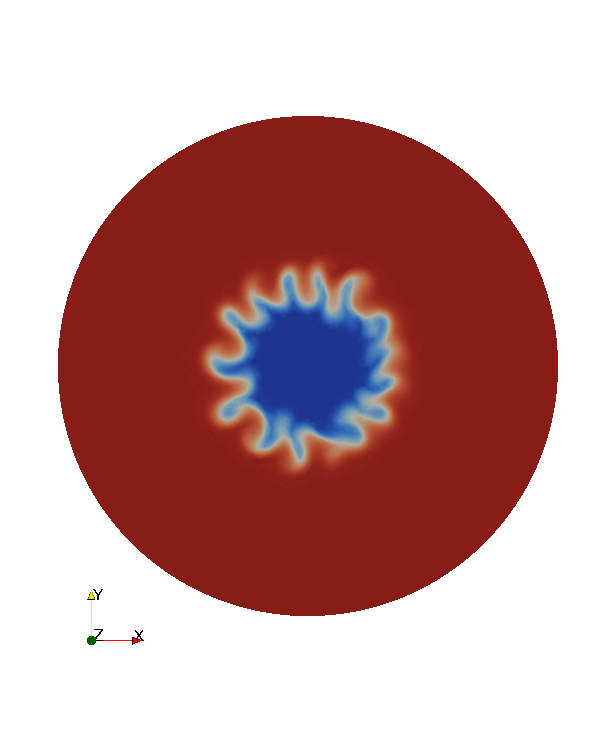
\includegraphics[width=0.175\textwidth]{./restratification_after_oodc/rousset-res5000-depth-40m0005.png}}
\subfigure [30 days]{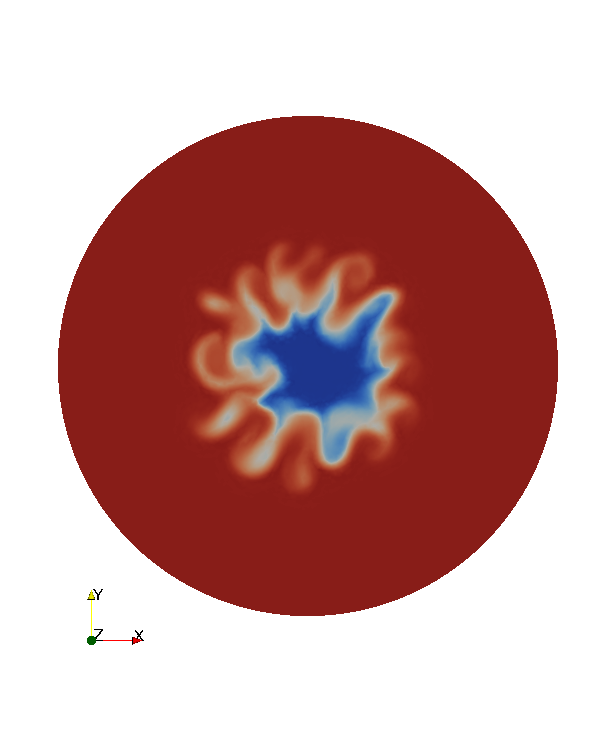
\includegraphics[width=0.175\textwidth]{./restratification_after_oodc/rousset-res5000-depth-40m0007.png}}
\subfigure [40 days]{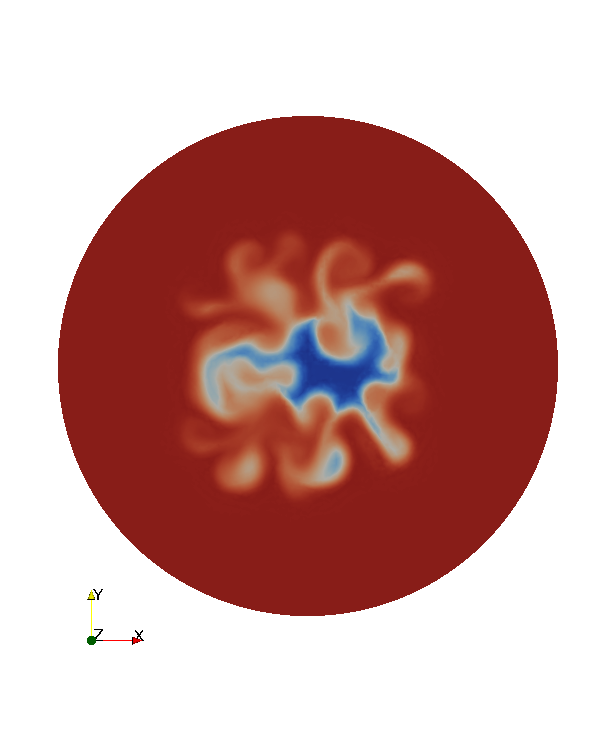
\includegraphics[width=0.175\textwidth]{./restratification_after_oodc/rousset-res5000-depth-40m0009.png}}
\caption{The temperature cross section at a depth of $40\,$m.}
\end{figure}
\end{frame}
%
\begin{frame}
    \frametitle{Restratification following open ocean deep convection, exercises}
\begin{itemize}
\item Work out the kinetic and potential energies using the vtus or stat file.
\item Try running with different resolutions and look at the effect on the eddies.
\end{itemize}
\end{frame}


%-- Add sections and your outline will be created automatically --%
\subsection{Tides in the Mediterranean Sea}

% Frame starts a new slide
\begin{frame}
    \frametitle{Tides in the Mediterranean Sea}
\begin{itemize}
\item Tidal modelling is a widely used method for validating free surface implementations.
\item Flow is driven by both astronomical and co-oscillating boundary tide forcing for the four main tidal constituents: \mbox{$M_2, \, S_2, \, K_1 \,\, {\rm and} \,\, O_1$}.
\item Run time: 5 hr. (64 cpu)
\end{itemize}
\end{frame}
%
\begin{frame}
    \frametitle{Tides in the Mediterranean Sea}
\begin{figure}
\centering
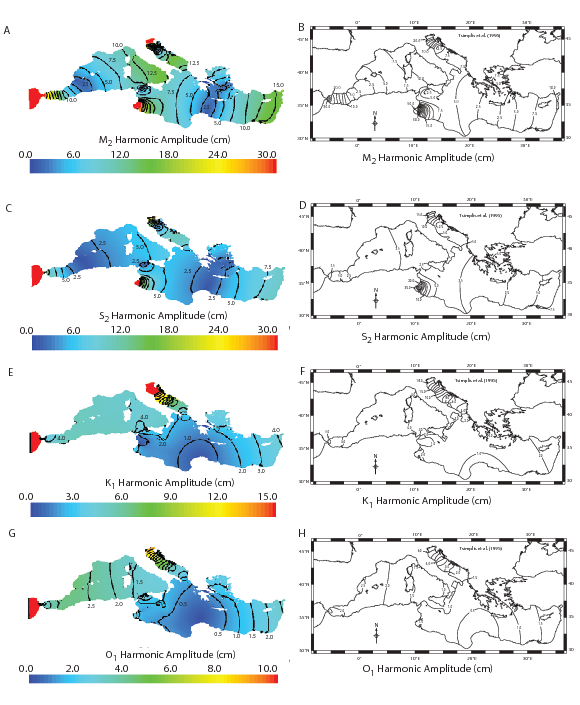
\includegraphics[width=0.9\textwidth, clip = True, trim = 5mm 180mm 0mm 0mm]{./tides_in_the_Mediterranean_Sea/amp.png}
\caption{Plots of the $M_2$ tidal harmonic amplitude in the Mediterranean Sea from Fluidity--ICOM and the high resolution
model of M. N. Tsimplis {\it et al.} (1995), J. Geophys. Res. 100(C8).}
\end{figure}
\end{frame}
%
\begin{frame}
    \frametitle{Tides in the Mediterranean Sea}
\begin{figure}
\centering
\includegraphics[width=0.6\textwidth]{./tides_in_the_Mediterranean_Sea/gauges.png}
\caption{Locations of 62 tide gauges in the Mediterranean Sea used to calculate the root mean square error.}
\end{figure}
\end{frame}



%-- Add sections and your outline will be created automatically --%
\subsection{Stokes square convection}

% Frame starts a new slide
\begin{frame}
    \frametitle{Stokes square convection}
\begin{itemize}
\item A steady–state isoviscous convection at a Rayleigh number (Ra) of $10^5$ , in a
  two dimensional square domain of unit dimensions 
\item comparison of numerical results against a well established two dimensional cartesian geometry
  benchmark result for Stokes flow
\end{itemize}
\end{frame}

\begin{frame}
    \frametitle{Stokes square convection}
\begin{figure}
  \includegraphics[width=0.5\textwidth]{./stokes_square_convection/Temperature_planform.png}
  \caption{Steady–state temperature field from an isoviscous Stokes simulation at $Ra = 1 \times
    10^5$, on a uniform structured mesh of 48 × 48 elements. Contours are spaced at intervals of
    0.1.}
\end{figure}
\end{frame}
%
\begin{frame}
    \frametitle{Stokes square convection}
\begin{figure}
\centering
\includegraphics[width=0.5\textwidth]{./stokes_square_convection/Nu_1e5.png}
\includegraphics[width=0.5\textwidth]{./stokes_square_convection/RMS_1e5.png}
\caption{Results from 2-D, isoviscous Stokes square convection benchmark cases: (a) Nusselt number
  vs. number of triangle vertices, at $Ra = 1 \times 10^5$, (b) RMS velocity vs. number of triangle
  vertices, at $Ra = 1 \times 10^5$ . Benchmark values are denoted by horizontal dashed lines. Note that the
  highest resolution case is not included in the example.}
\end{figure}
\end{frame}
%
\begin{frame}
    \frametitle{Stokes square convection, exercises}
\begin{itemize}
\item Verify that results do indeed converge towards the benchmark values at higher resolution.
\item Alter the initial condition for temperature to verify that, excluding the location of upwelling
flow at $x = 0$ or $x = 1$, results are insensitive to this initial condition.
\item Change the Rayleigh number to $Ra = 1 \times 10^4$
\end{itemize}
\end{frame}



\section*{Getting started}
\begin{frame}
  \frametitle{Getting started}
  \begin{itemize}
  \item The examples have been run in advance and the output can be found in \texttt{/scratch/examples}
  \item You may need to specify your Fluidity binaries folder \\
    \texttt{export PATH=<<fluidity dir>>/bin/:\$PATH}
  \item and Python tools folder \\
    \texttt{export PYTHONPATH=<<fluidity dir>>/python/:\$PYTHONPATH}
  \item If you get `permission denied' running a postprocessing script, try \\
    \texttt{chmod u+x <<script>>}
  \end{itemize}
\end{frame}

\end{document}




